@@ -0,0 +1,770 @@
\chapter{TPC Electronics}
\label{ch:fddp-tpc-elec}


%%%%%%%%%%%%%%%%%%%%%%%%%%%%%%%%%%%%%%%%%%%%%%%%%%%%%%%%%%%%%%%%%%%%
\section{TPC Electronics System Overview}
\label{sec:fddp-tpc-elec-ov}

%%%%%%%%%%%%%%%%%%%%%%%%%%%%%%%%%
\subsection{Introduction}
\label{sec:fddp-tpc-elec-intro}

The aim of the \dword{dp} TPC electronics is to collect and digitize the signals from the %Charge Readout Planes 
(\dwords{crp}) and \dwords{pd} %photon detectors, 
photomultiplier tubes (\dword{pmt}), in the Dual-Phase (\dword{dp}) detector module. 
\fixme{something about its components: the \dword{cro} and the LRO}

The design of the system incorporates the components already developed for the \Dword{pddp} as a result of an R\&D activity started in 2006. One of the key objectives of this R\&D program has been the design of an electronics system that is easily scalable and cost-effective in order to meet the needs of the large-scale \dword{dpmod}. % neutrino \dword{lar} detector.  

\fixme{you need a figure here - schematic maybe - showing the system and how it fits in with the other systems (anne)}

While a single \dword{dpmod} has a factor of \num{20} more readout (both charge and light) channels than \dword{pddp}, a simple scaling of the number of the components used in the prototype design is sufficient to meet these needs without necessitating any additional R\&D. A small-scale version of the TPC electronics system was used in a preliminary \dual \lartpc prototype, \dword{wa105},  at CERN with an active volume  of \SI[product-units=power]{3x1x1}{m} (\dword{crp} area of \SI[product-units=power]{3x1}{m}) that took data in the summer-fall of 2017. %The experience gained from the \dword{wa105} operation allowed to validate already some of the design choices and check various performance markers (e.g., noise). 
Operation of the \dword{wa105} validatated some of the design choices and provided checks on various performance markers (e.g., noise). 

The \dword{cro} system is designed to provide continuous, non-zero-suppressed, and losslessly compressed digital signals by reading the charge collected on the \dwords{crp}' \SI{3}{m} long strips that are arranged in two collection views, all with a pitch of \SI{3.125}{mm}.% in the \dword{crp}. 
The system consists of %a 
the \dword{fe} analog electronics operating at cryogenic temperatures and digital electronics working in the warm environment outside of the cryostat.  The cryogenic \dshort{fe} analog electronics is based on an application-specific integrated circuit (ASIC) chip with a large dynamic range (up to \SI{1200}{fC}) to cope with the charge amplification in the \dwords{crp}. The analog \dword{fe} cards are housed in dedicated signal feedthrough (\dword{sft}) chimneys and are accessible from the outside even after the \dword{dpmod} is in operation, thus removing any significant risks associated with their long-term survivability. The \dword{sft} chimneys are approximately \SI{2.3}{m} long objects that traverse the entire insulation layer of the cryostat allowing placement of the \dword{fe} electronics close to the \dword{crp} to minimize cable capacitance (noise).  In addition, their metallic structure shields the \dword{fe} cards 
\fixme{\dword{fe} cards not defined; also need image}
from any interference from the digital electronics and ambient environment. The analog signals are digitized by \dwords{amc}, which are housed in the commercial uTCA crates on top of the cryostat near the \dword{sft} chimneys. 

The data are sampled at the rate of \SI{2.5}{MHz} with \SI{12}{bit} resolution.  This frequency, traditionally used in \lartpc experiments, is well matched to the \SI{1}{\micro\second} pulse-shaping time of the \dword{fe} electronics and the detector response times determined by the electron drift velocity in the \lar. The corresponding sampling resolution along the drift coordinate is better than \SI{1}{\mm}. 

The \dword{lro} electronics collects and digitizes the signals from the \dword{pds}, which consists of \dword{tpb}-coated \num{8}\,in \dwords{pmt} (Hamamatsu\footnote{Hamamatsu\texttrademark R5912-02-mod} R5912-02-mod) located beneath the TPC cathode. The \dword{lro} electronics %should 
facilitates the detection of the primary scintillation signals, which provide the absolute time reference for the interaction events. It %should 
also enables recording the light signals generated by photons from the so-called \textit{proportional scintillation component}, the light created by the electrons extracted and amplified in the gaseous phase. 
\fixme{what detection element is up there?} The electronics, consisting of analog and digital stages, is housed in the uTCA crates on top of the cryostat structure. The card design shares a similar architecture with the AMCs for the charge readout. 

Each uTCA crate for either charge or light readout is connected to the \dword{daq} system via an optical fiber link that supports at least \SI{10}{Gbit/s}. Every crate also contains a %module, 
\dword{wrmch} for the time synchronization of the digital electronics. This timing slave unit is connected via \SI{1}{Gbit/s} optical fiber to a master node that serves as a synchronization reference for all the connected slave nodes on the network. This system for the time synchronization is based on the commercially available components developed within the framework of the White Rabbit (\dword{wr}) project with ad-hoc hardware and firmware developments. The system performs automatic and continuous self-calibrations to account for any propagation delays and is able to provide sub-\si{\nano\s} accuracy for the timing synchronization.


%%%%%%%%%%%%%%%%%%%%%%%%%%%%%%%%%%%%%
\subsection{Design Considerations}
\label{sec:fddp-tpc-elec-des-consid}

%The principal requirements for the DP TPC electronics system can be summarized as:

The design of the electronics for the charge readout covers the analog \dword{fe} cards containing pre-amplifier ASICs operating at cryogenic temperatures and digitization cards with the relevant system for their synchronization working in the warm environment outside of the cryostat. The system %should 
reads and digitizes signals from a total of \num{153600} channels (per one \dword{dpmod}) and be capable of continuously streaming the collected and losslessly compressed data to the \dword{daq} without any zero suppression. 
The design of the \dshort{cro} electronics system was developed to fit the following requirements:
\begin{itemize}
\item{The \dword{cro} electronics %must be able to 
shall measure signals of up to \SI{1200}{\femto\coulomb} without saturation; this has been optimized following \dword{mc} studies on the maximal occupancy per channel in shower events~\cite{WA105_TDR}. For a nominal \dword{crp} gain of \num{20}, a \dword{mip} signal is expected to be around \SI{30}{fC} -- the lowest limit that assumes a particle travelling horizontally with an azimuthal angle of \num{0} degrees -- giving %the 
a maximal operational range of up to \num{40} \dwords{mip}.}

\item{The electronic noise in the \dshort{cro} analog electronics is required to be \SI{<2500}{e^{-}}. This condition can be derived from the requirement on the minimal \dword{s/n}, which should be greater than \num{5}:\num{1} once the charge attenuation is taken into account. Given the maximum drift distance of \SI{12}{\meter}, the largest attenuation factor due to electro-negative impurities assuming the \SI{3}{\milli\second} (minimally required) electron lifetime and the drift field of \SI{0.5}{\kilo\volt/\cm} is \num{0.08}. The smallest \dword{mip} signal with the \dword{crp} effective gain of \num{20} is therefore \SI{2.5}{\femto\coulomb} (\SI{15600}{e^{-}}).}

\item{The peaking time of the \dword{fe} analog amplifiers %should 
shall be \SI{1}{\micro\second}. This requirement is driven by the the need for optimal vertex resolution, determined in turn by the single track resolution and the power to separate two or more tracks that are close to one another.}

\item{The sampling frequency %should 
shall be \SI{2.5}{\MHz} to match the peaking time of the \dword{fe} electronics.}

\item{The power dissipated by the \dword{fe} analog electronics %must 
shall be below \SI{50}{\milli\watt/channel} in order to minimize the heat input to the cryostat volume.}

\item{The \dword{fe} analog electronics %should 
shall be replaceable without the risk of contaminating the main \lar volume in order to guarantee the long-term reliability of the system.}

\item{The \dword{adc} resolution %should 
shall be such that that the noise is at 
\fixme{does not exceed?} the level of an \dword{adc}, %while 
given a dynamic range wide enough to match the response of the \dword{fe} amplifier. This can be achieved with a \num{12} bit \dword{adc}.}

\item{The digital electronics to be placed outside of the cryostat in the warm environment %can 
shall be capable of adopting standard industrial components and solutions, to keep the costs lower and to benefit from  %ensuring low costs and benefiting of the 
technological evolution (e.g., higher network speeds).}
\end{itemize}
As described in the details in subsequent sections, the performance of the final system is significantly better with respect to many of the listed aspects.  \fixme{above sentence not needed (anne)}

The magnitude of the noise also %plays a role in 
has an effect on the quality of the lossless compression of the raw data.% performed by the digital electronics. 
A compression factor of about \num{10} could be achieved with the RMS noise level below \SI{1}{\dword{adc}}, while with the noise at around \SI{1.5}{\dword{adc}} the compression factor of \num{4} is obtained. 
\fixme{What are you saying here: ``we're expecting 1.5 ADC so we'll only get factor of 4, but wouldn't it be nice to get factor of 10''? If that's your meaning, what's keeping you from getting the noise low enough?}
% A compression factor of \num{7} can be achieved with a RMS noise level of $\sim$ \SI{1.5}{\dword{adc}}, increasing to \num{10} for RMS noise levels below \SI{1}{\dword{adc}} RMS.

%Given the amplification of the ionization charge in \dword{crp}, the electronics needs to be sensitive to the signals over a large dynamic range (up-to \num{40} times the \dword{mip}-level signals for a nominal \dword{crp} gain of %\num{20} or \SI{1200}{\femto\coulomb}) to avoid saturation of the analog inputs by large localized energy disposition produced, for example, in shower events. The minimal requirelemt on the intrinsic noise %of the \dword{fe} analog electronics is \SI{<2500}{e^{-}}.  The condition is derived from the requirement on the minimal \dword{s/n} of \num{5:1} as in the SP design. Given the maximal drift \SI{12}{\meter} the %largest attenuation factor due to electro-negative impurities assuming the nominal \SI{3}{\milli\second} electron lifetime is \num{0.08}. The smallest \dword{mip} signal with the \dword{crp} effective gain is therefore %\SI{2.5}{\femto\coulomb} (\SI{15600}{e^{-}}).

%The charge amplification provided by the \dword{crp} loosens requirements on the intrinsic noise of the \dword{fe} analog electronics. For the \dword{crp} nominal gain of \num{20}, the signal-to-noise ratio for a \dword{mip} signal %(\SI{30}{fC}) should be around \num{100}, which would not pose any problems for the detection/reconstruction. 

The primary objective of the \dword{lro} system is to detect signals, from a minimum of one photo-electron on one \dword{pmt}, giving a precise timestamp that can be used in conjunction with the charge signals to determine the time (drift) coordinate of an event. \fixme{why insert (drift)?}  Precise measurements of signal charge allow the continual monitoring of the \dword{pmt} gain at the single photo-electron level, and the determination of the number of photons in each scintillation event.  In addition, an \dword{adc}  continuously streams data, downsampled to \SI{400}{ns} as for the \dword{cro} signals,  which, amongst other items, allows measurements of the scintillation time profile. In addition, the \dword{lro} system samples a small number of signals from the \dword{pd} calibration system: the calibration trigger and around \num{20} channels from reference sensors.

The cryogenic analog electronics for the \dword{cro} is housed in the dedicated \dword{sft} chimneys. %Their 
Its design must enable access to the \dword{fe} card for possible replacement without any risk of contaminating the pure \lar in the main cryostat volume. The chimneys must possess a cooling system that can control the temperature around the \dword{fe} cards to roughly \SI{110}{\kelvin} %for their optimal noise. 
to reach their optimal noise level. In addition, the cooling system must compensate for the heat input from the chimneys into the cryostat volume. \fixme{are chimneys part of this system?}

The digital electronics for both charge and light readout is located in the warm environment on the top of the cryostat supporting structure and is therefore easily accessible. This fact removes any constraints associated with the accessibility and operation in cryogenic environments allowing for the usage of standard components and industrial solutions in the design. Digital electronics must be continuously and automatically synchronized to better than \SI{400}{\nano\s} to ensure the correct temporal alignment of the \dword{adc} samples from all of the readout channels. This is a minimal requirement dictated by the fact that the sampling rate is \SI{2.5}{\MHz}.  

\begin{dunetable}
[Parameters for the TPC electronics system design]
{lr}
{tab:dpele-physicsparams}
{Parameters for the  TPC electronics system design. The numbers are given for one detector module.}   
Parameter & Value  \\ \toprowrule
  \dword{cro} channels    &  \num{153600}            \\ \colhline
  \dword{cro} continuous sampling rate & \SI{2.5}{\MHz}\\ \colhline
  \dword{cro} \dword{adc} resolution & \num{12} bit           \\ \colhline
  \dword{cro} data compression factor   & \num{10}    \\ \colhline 
  \dword{cro} data flow  & \num{430} Gibit/s          \\ \colhline 
  LRO channels       & \num{720}               \\ \colhline
  LRO continuous sampling rate & \SI{2.5}{\MHz} \\ \colhline
  LRO \dword{adc} resolution & \num{14} bit            \\ \colhline
  LRO data compression factor  & \num{1}       \\ \colhline
  LRO data flow   & \num{24} Gibit/s          \\ \colhline
\end{dunetable}

Some of the key parameters in the electronics system design are summarized in Table~\ref{tab:dpele-physicsparams}. %The requirements for the DP electronics system are documented in DUNE-docdb-6428.


%%%%%%%%%%%%%%%%%%%%%%%%%%%%%%%%
\subsection{Scope}
\label{sec:fddp-tpc-elec-scope}

The scope of the TPC electronics system covers the procurement and productions, testing and validation, installation, and commissioning of all the components necessary to ensure the complete readout of the charge and light signals from a given DP detector module. The covered items are the following:
\begin{itemize}
\item{Cryogenic analog \dword{fe} cards for charge readout}
\item{AMC cards for charge/light readout}
\item{The WR-MCH cards for AMC clock synchronization}
\item{uTCA crates}
\item{Switches for the White Rabbit network}
\item{\dword{sft} chimneys}
\item{Low-voltage power supplies, distribution, and filtering system for the \dword{fe} cards}
\item{Flat cables connecting the \dword{fe} cards to the warm flange interface of the \dword{sft} chimneys}
\item{VHDCI cables connecting the warm flange interface of the \dword{sft} chimneys to AMCs}
\end{itemize}

The total numbers for components to be procured to instrument one detector module are given in Table~\ref{tab:dpele-num-components}

\begin{dunetable}
[Numbers for DP electronics components to procure]
{lr} {tab:dpele-num-components}
{Numbers for DP electronics components to procure for one detector module.}
Name & Number  \\ \toprowrule
\dword{cro} cryogenic ASICs (\num{16} ch) & \num{9600} \\ \colhline
\dword{cro} cryogenic analog \dword{fe} cards (\num{64} ch) & \num{2400} \\ \colhline
\dword{cro} AMCs & \num{2400} \\ \colhline
\dword{sft} chimneys & \num{240} \\ \colhline
Flat cables for \dword{sft} chimney (\num{68} ch) & \num{2400} \\ \colhline
Flat cables for \dword{sft} chimney (\num{80} ch) & \num{2400} \\ \colhline
VHDCI cables (\num{32} ch) & \num{4800} \\ \colhline
LRO AMCs with analog \dword{fe} & \num{45} \\ \colhline
uTCA crates & \num{245} \\ \colhline
WR-MCH units & \num{245} \\ \colhline
WR switches (\num{18} ports) & \num{16} \\ \colhline
\end{dunetable}


%%%%%%%%%%%%%%%%%%%%%%%%%%%%%%%%%%%%%%%%%%%%%%%%%%%%%%%%%%%%%%%%%%%%
\section{TPC Electronics System Design}
\label{sec:fddp-tpc-elec-design}

The \dword{cro} \dword{fe} analog electronics is based on cryogenic ASIC chip with a large dynamic range (up to \SI{1200}{\femto\coulomb}) to accomodate the charge amplification in the dual-phase \dword{crp}. The \dword{fe} cards read \num{64} \dword{crp} channels each. They are mounted in dedicated Signal FeedThrough (\dword{sft}) chimneys and are located within a short distance (\SI{<1}{\metre}) from each \dword{crp} to minimize the noise caused by long cables (large cable capacitance). The cards remain accessible throughout the detector operation. Each \dword{sft} chimney hosts \num{10} \dword{fe} analog cards, which corresponds to the readout of \num{640} \dword{crp} channels per chimney. There are, therefore, \num{240} \dword{sft} chimneys to be installed for the charge readout in a given DP detector module.   

The differential analog signals from the analog \dword{fe} cards, carried by the twisted-pair ribbon cables and routed via an interface flange of the \dword{sft} chimneys, are digitized by the AMC cards located in the warm conditions outside of the cryostat. These cards are hosted in uTCA crates placed in the immediate vicinity of the \dword{sft} chimneys (one crate per chimney). In the baseline version of the design currently used for \dword{pddp}, each AMC digitizes \num{64} channels corresponding to reading one \dword{fe} analog card. Each uTCA in such case contains \num{10} AMCs reading a total of \num{640} channels. However, an implementation with AMCs supporting a higher channel density is also being investigated for cost reduction purposes.

The LRO \dword{fe} analog and digital electronics is based on a custom-built AMC. The card contains a \dword{catiroc} ASIC, which is used to determine precisely the charge and start times of signals from each individual \dword{pmt}. In addition, a \SI{14}{bit} \SI{65}{MHz} \dword{adc} digitizes the data for continuous streaming of the \dword{pmt} signals. Each card can read up to \num{16} channels. A potential future upgrade is to increase the channel density per card to \num{32} channels. The LRO cards are housed in five dedicated uTCA crates located close to the \dword{pmt} instrumentation feedthroughs.

\begin{dunefigure}[Top view of DP detector module]{fig:dpele-sft-chimney-pattern}
{Corner view of DP detector module showing the pattern of the \dword{sft} chimneys and uTCA crates for charge readout above CRPs.}
\includegraphics[width=0.6\textwidth]{dpele-sft-chimney-pattern}
\end{dunefigure}

Every uTCA crates contains a network switch, MicroTCA Carrier Hub (\dword{mch}), via which the data are sent to \dword{daq} as well as a module (\dword{wrmch}) for clock/time synchronization and trigger timestamp distribution to the AMCs. Both MCH and WR-MCH require one optical fiber link each. 

The MCH switch streams the data from AMCs via a dedicated optical link. Currently \dword{pddp} uses MCH operating at \SI{10}{Gbit/s}. However, a move to \SI{40}{Gbit/s} links for the DUNE FD implementation is considered because of the technology evolution with associated cost reductions and possible increase in the channel density of each AMC.

The WR-MCH time synchronization unit is based on the White Rabbit (WR) system, which provides hardware and protocols for the network-based sub-ns synchronization between a master and different slave nodes. The connection of the WR-MCH to the White Rabbit network is done via \SI{1}{Gbit/s} synchronous Ethernet optical link. WR-MCH distributes the timing information for synchronization of the AMCs via the uTCA backplane. In addition, this unit can be used to transmit triggers to the digitization units within the crate. This is achieved by sending it dedicated data packets containing trigger timestamp information. 

Figure~\ref{fig:dpele-sft-chimney-pattern} shows a corner view of the DP detector module illustrating the pattern of the \dword{sft} chimneys and the attached uTCA crates above the CRPs. Each crate/\dword{sft} chimney collects signals from \SI{3}{\meter} long strips of two \SI[product-units=power]{1x3}{\meter} \dword{crp} segments. Each chimney completely traverses the insulation layers (not shown in the figure). 
%A cut-out view of the chimney illustrates the location of the \dword{fe} cards and provides the overall scale of this object. 


\begin{dunetable}
[Summary of some of the principal numbers of the TPC electronics system.]
{lr} {tab:dpele-numparts}
{Summary of some of the principal numbers of the TPC electronics system for charge and light readout of a detector module.}
Name & Number  \\ \toprowrule
   \dword{cro} \dword{sft} chimneys/uTCA crates              &  \num{240}   \\ \colhline
   \dword{cro} channels per \dword{sft} chimney/uTCA crate & \num{640} \\ \colhline
   \dword{cro} cryogenic analog \dword{fe} cards per \dword{sft} chimney    &  \num{10}     \\ \colhline
%   \dword{cro} Cryogenic analog \dword{fe} cards (total)                   & \num{2400}  \\ \colhline
   \dword{cro} AMCs per uTCA crate                       & \num{10}      \\ \colhline
%   Charge readout AMCs (total)                                   & \num{2400}      \\ \colhline 
   LRO \dword{fe} cards  per uTCA crate & \num{9} \\ \colhline
%   Light readout \dword{fe} cards (total)           & \num{45} \\ \colhline
   LRO channels per uTCA crate & \num{144} \\ \colhline
   LRO uTCA crate                      & \num{5} \\ \colhline
   WR-MCH per uTCA crate                 & \num{1} \\ \colhline
%   WR-MCH (total)                              & \num{245} \\ \colhline
%   uTCA crates (total)                         & \num{245} \\ \colhline
\end{dunetable}

A short summary of some of  the number of principal components and channel granularity in the design of the DP electronics is provided in Table~\ref{tab:dpele-numparts}. 

%%%%%%%%%%%%%%%%%%%%%%%%%%%%%%%%%%%
\subsection{Cryogenic Analog \dword{fe} Electronics}
\label{sec:fddp-tpc-elec-design-cryofe}

The cryogenic amplifier ASIC is the main component of the \dword{fe} analog cards. Its design is based on the CMOS \SI{0.35}{\micro\meter} technology and is an outcome of an R\&D  activity started in 2006, which resulted in several versions of the cryogenic amplifier for both single and dual-phase \dword{lartpc} detectors. Two principal versions of ASIC chips have been produced for the dual-phase \dword{lartpc} operation. In the first version the amplifiers have a constant gain in the region of $0-1200$ \si{\femto\coulomb} ($0-40$ \dword{mip}). In the second, the amplifiers have a higher linear gain for signals up to \SI{400}{\femto\coulomb} (roughly 10 \dword{mip} signals) and a logarithmic response in the $400-1200$ \si{\femto\coulomb} range. This double-slope behavior is obtained by using a MOSCAP capacitor in the feedback loop of the amplifier that changes its capacitance above a certain signal threshold. The aim of this solution is to optimize the resolution for small charge depositions (in a few \dword{mip} region) while preserving overall the large dynamic range of the amplifier.

\begin{dunefigure}[Cryogenic \dword{fe} ASIC properties]{fig:dpele-fe-asic-prop}
{Cryogenic \dword{fe} ASIC properties: amplifier response (left) and noise (right) at different temperatures measured at the output of differential buffer.}
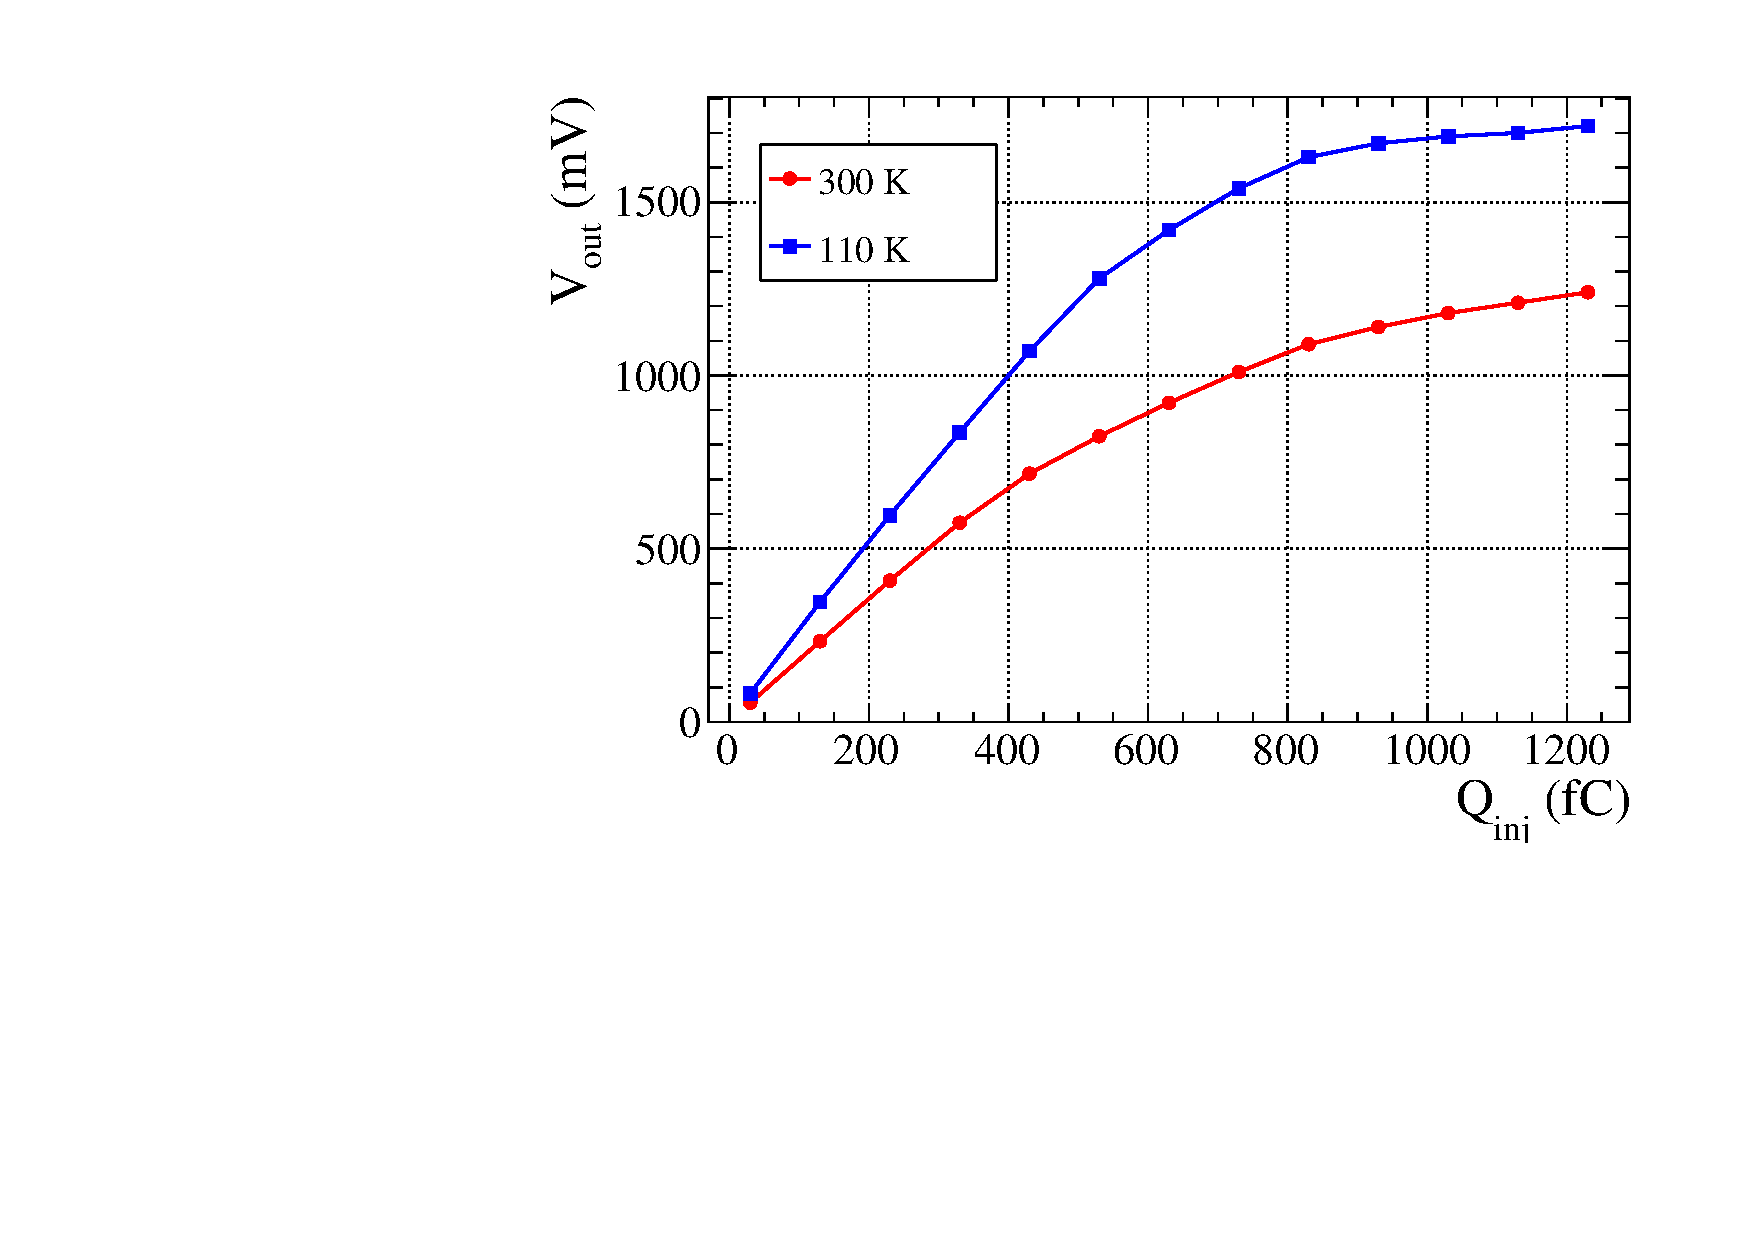
\includegraphics[width=0.49\textwidth]{dpele-fe-asic-gain}
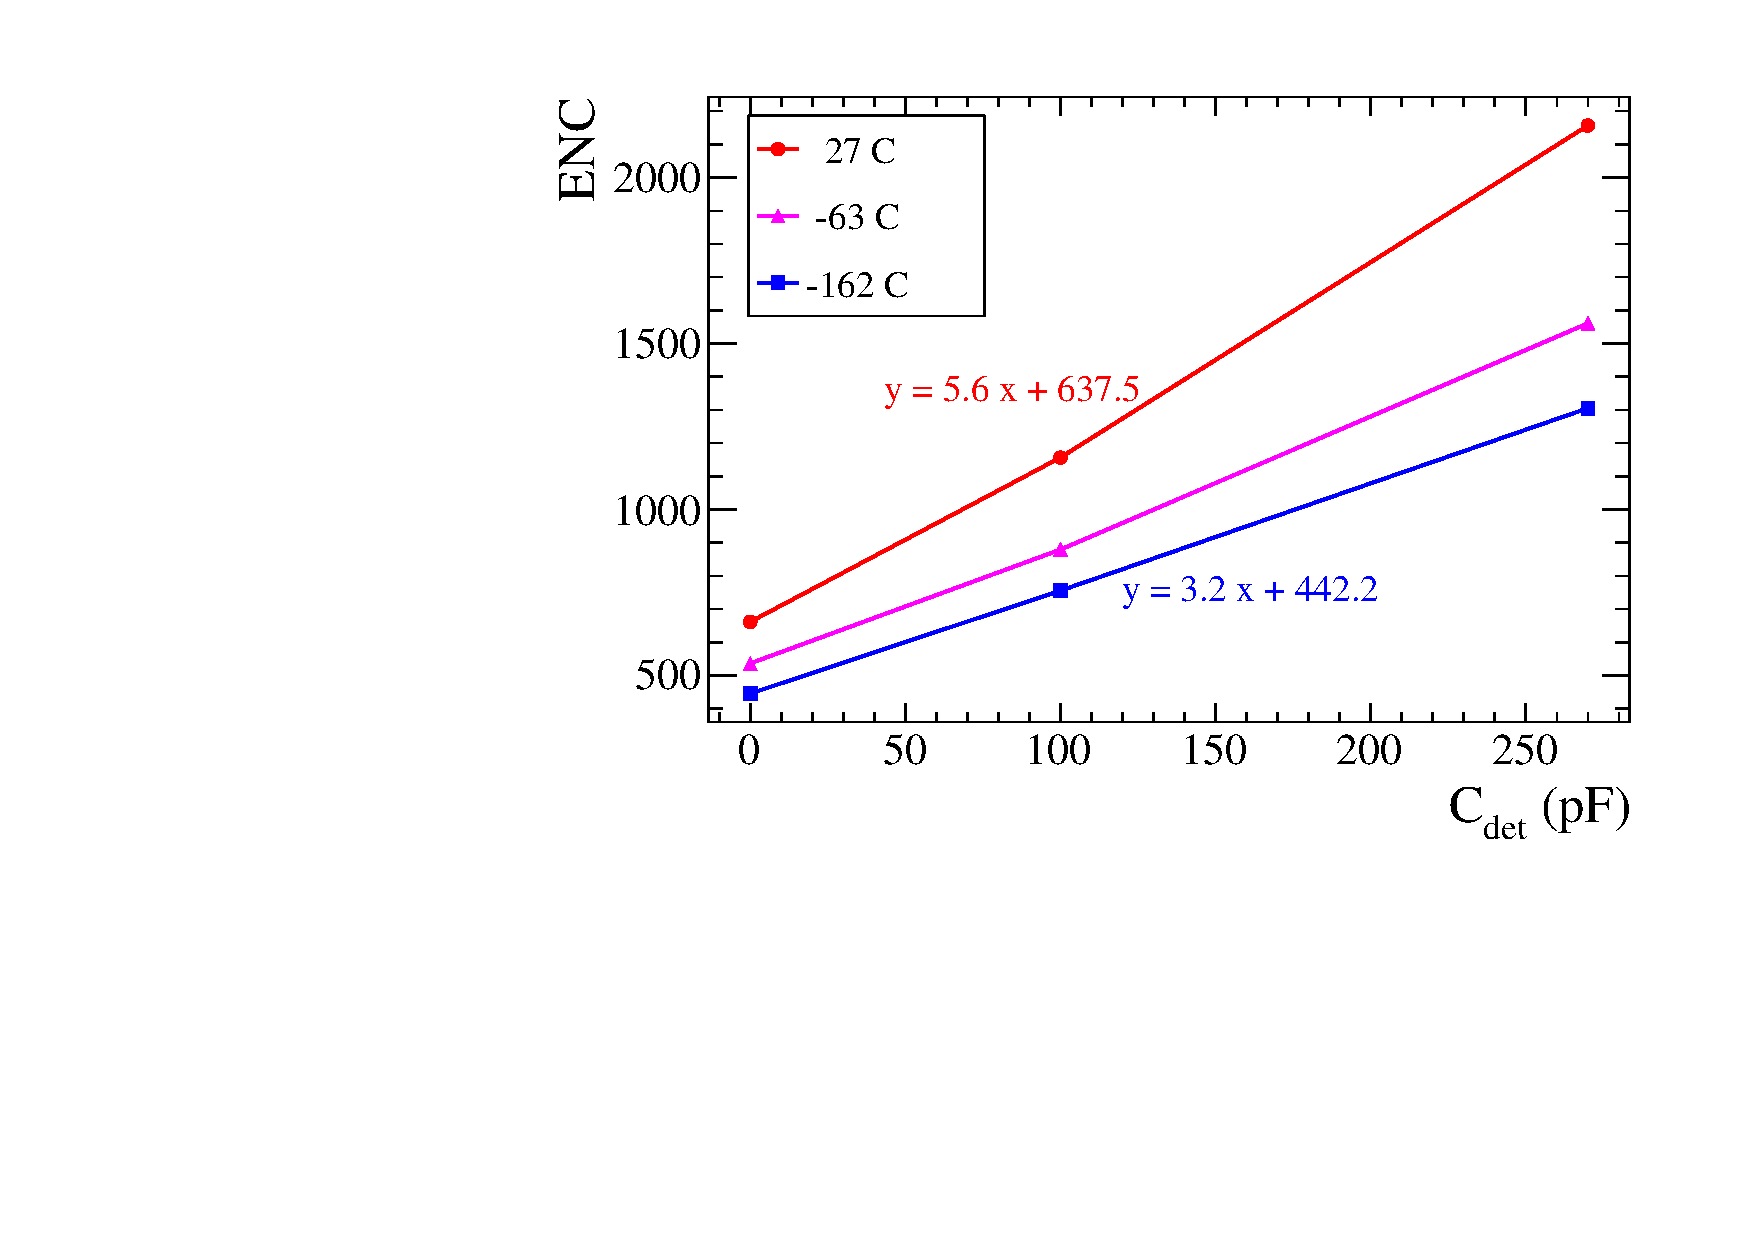
\includegraphics[width=0.49\textwidth]{dpele-fe-asic-noise}
\end{dunefigure}

%Figure~\ref{fig:dpele-fe-asic-noise} 
The ASIC version with the double-slope gain has been selected for \dword{pddp} and adopted for the DP TPC electronics design. The left plot in Figure~\ref{fig:dpele-fe-asic-prop} illustrates the response of this amplifier for different values of the injected charge, while that on the right shows the measured noise in units of Equivalent Noise Charge (ENC) as a function of the "detector" capacitance at different temperatures. For the \dword{crp} anode (detector) capacitance of \SI{480}{\pico\farad} per \SI{3}{\metre} strip, the expected noise is around \SI{2000}{e^{-}} at \SI{110}{\kelvin}. Each ASIC contains \num{16} amplifier channels with differential line buffers and has a power consumption, which is \SI{11}{\milli\watt/channel} surpassing the \SI{<50}{\milli\watt/channel} requirement. 

\begin{dunefigure}[Image of an analog \dword{fe} card mounted on the extraction blade]{fig:dpele-fe-card-blade-image}
{Image of an analog cryogenic \dword{fe} card mounted on the extraction blade.}
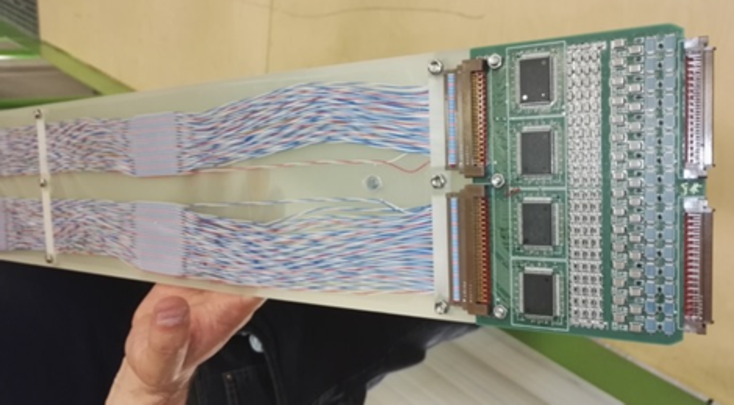
\includegraphics[width=0.7\textwidth]{dpele-fe-card-blade-image}
\end{dunefigure}

Each cryogenic \dword{fe} card, shown in Figure~\ref{fig:dpele-fe-card-blade-image}, hosts four ASIC amplifier chips and a few passive discrete components. The input stage of each amplifier channel has a \SI{1}{\giga\ohm} resistor to ground followed by a \SI{2.2}{\nano\farad} decoupling capacitor; both are rated for HV operation. The function of the resistor is to ground the \dword{crp} anode strips. Each input stage is also protected against discharges coming from the detector with a TVS diode (Bourns CDSOD323-T08LC). This component was selected after studying the performance of different devices for the electrostatic discharge protection by subjecting them systematically to discharges of a few kV with an energy similar to that of the Large Electron Multipliers (LEMs) in the \dword{crp}. The \dword{fe} cards also house the blocking capacitors for further filtering of the low voltage power lines. These are first filtered at the level of the power supply and transported with shielded cables.

\begin{dunefigure}[Noise measurements in \dword{wa105} in different conditions]{fig:dpele-311-noise}
{Noise of measurements in \dword{wa105} in different conditions. Left: at warm with the slow control cables connected to the cryostat flanges (red points) and disconnected (black points). Right: at warm (red points) and cold (black points) with the slow control cables disconnected. The channels with negative (positive) channel number correspond to the strips of \SI{3}{\meter} (\SI{1}{\meter}).}
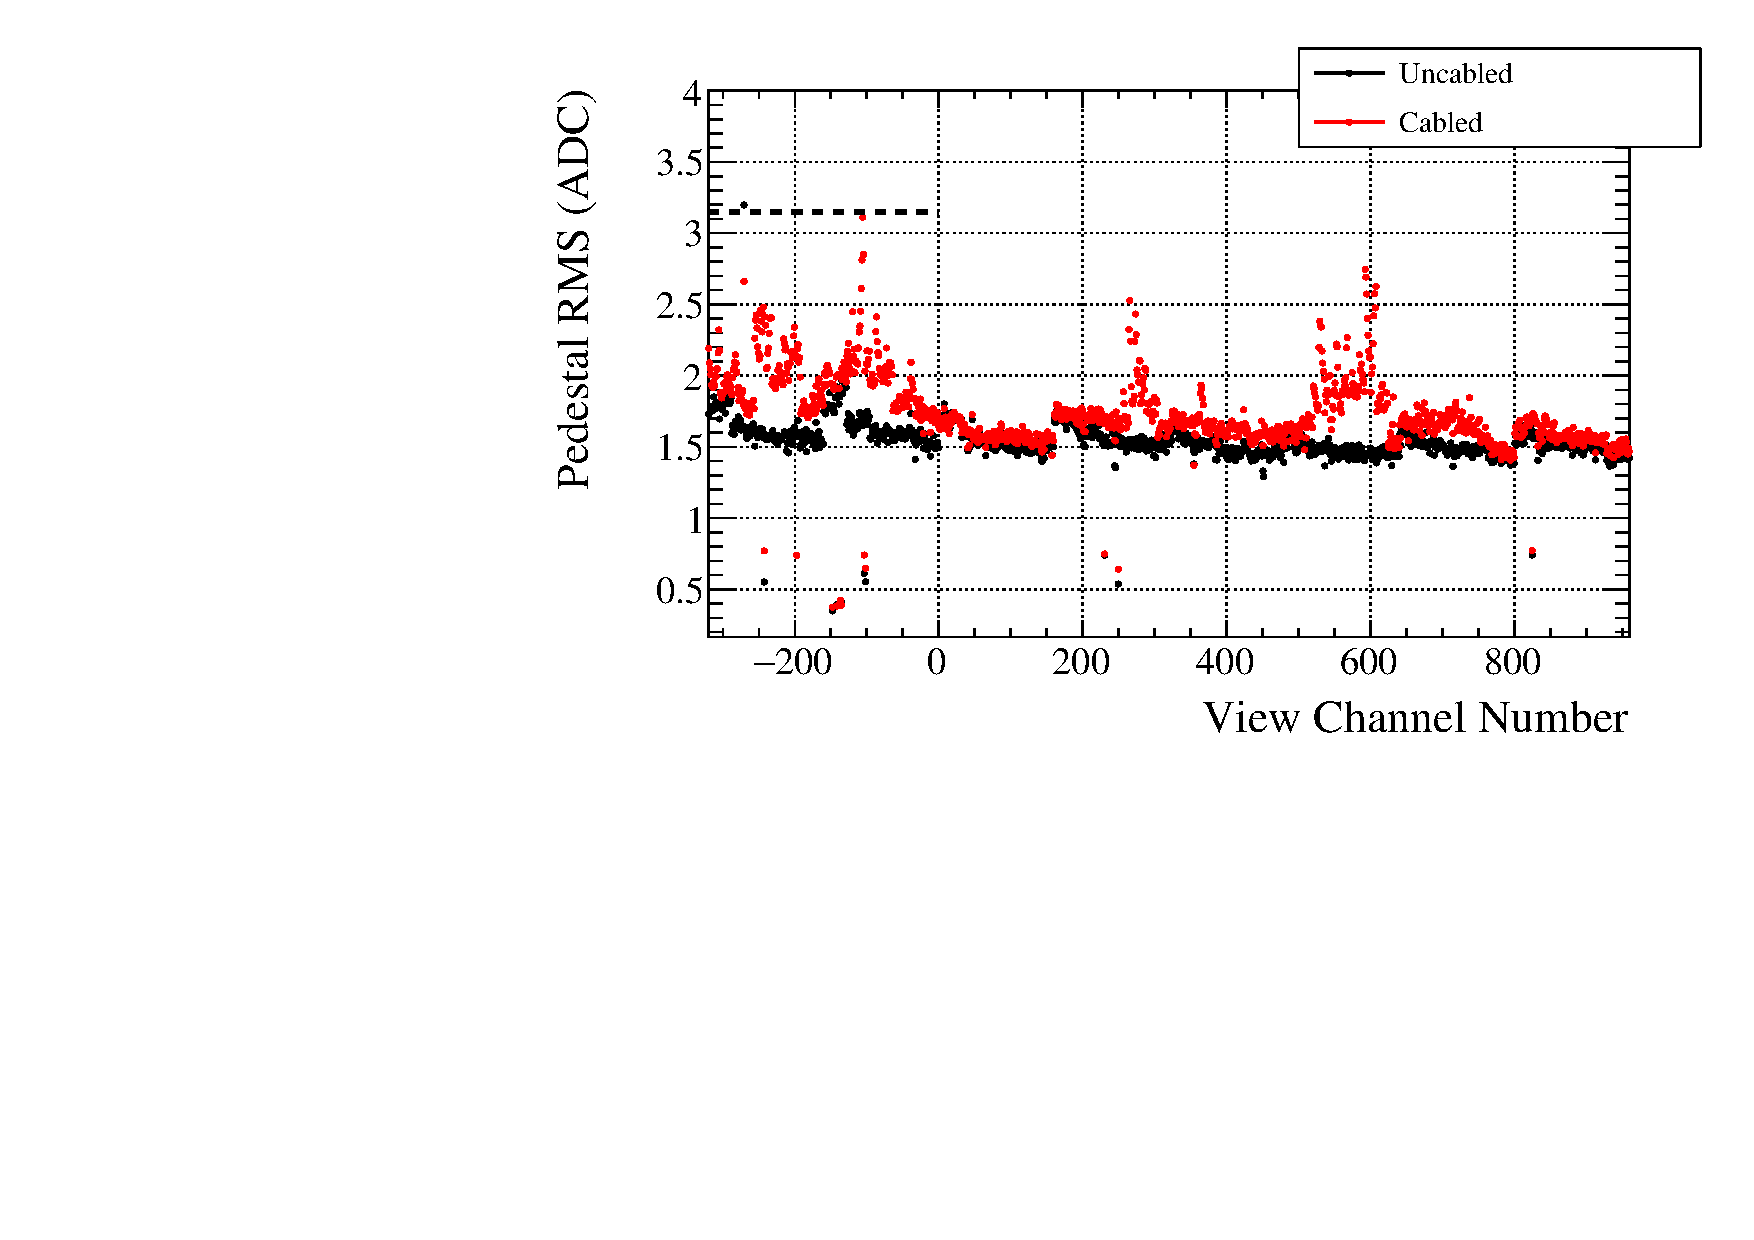
\includegraphics[width=0.45\textwidth]{dpele-311-noise-warm}
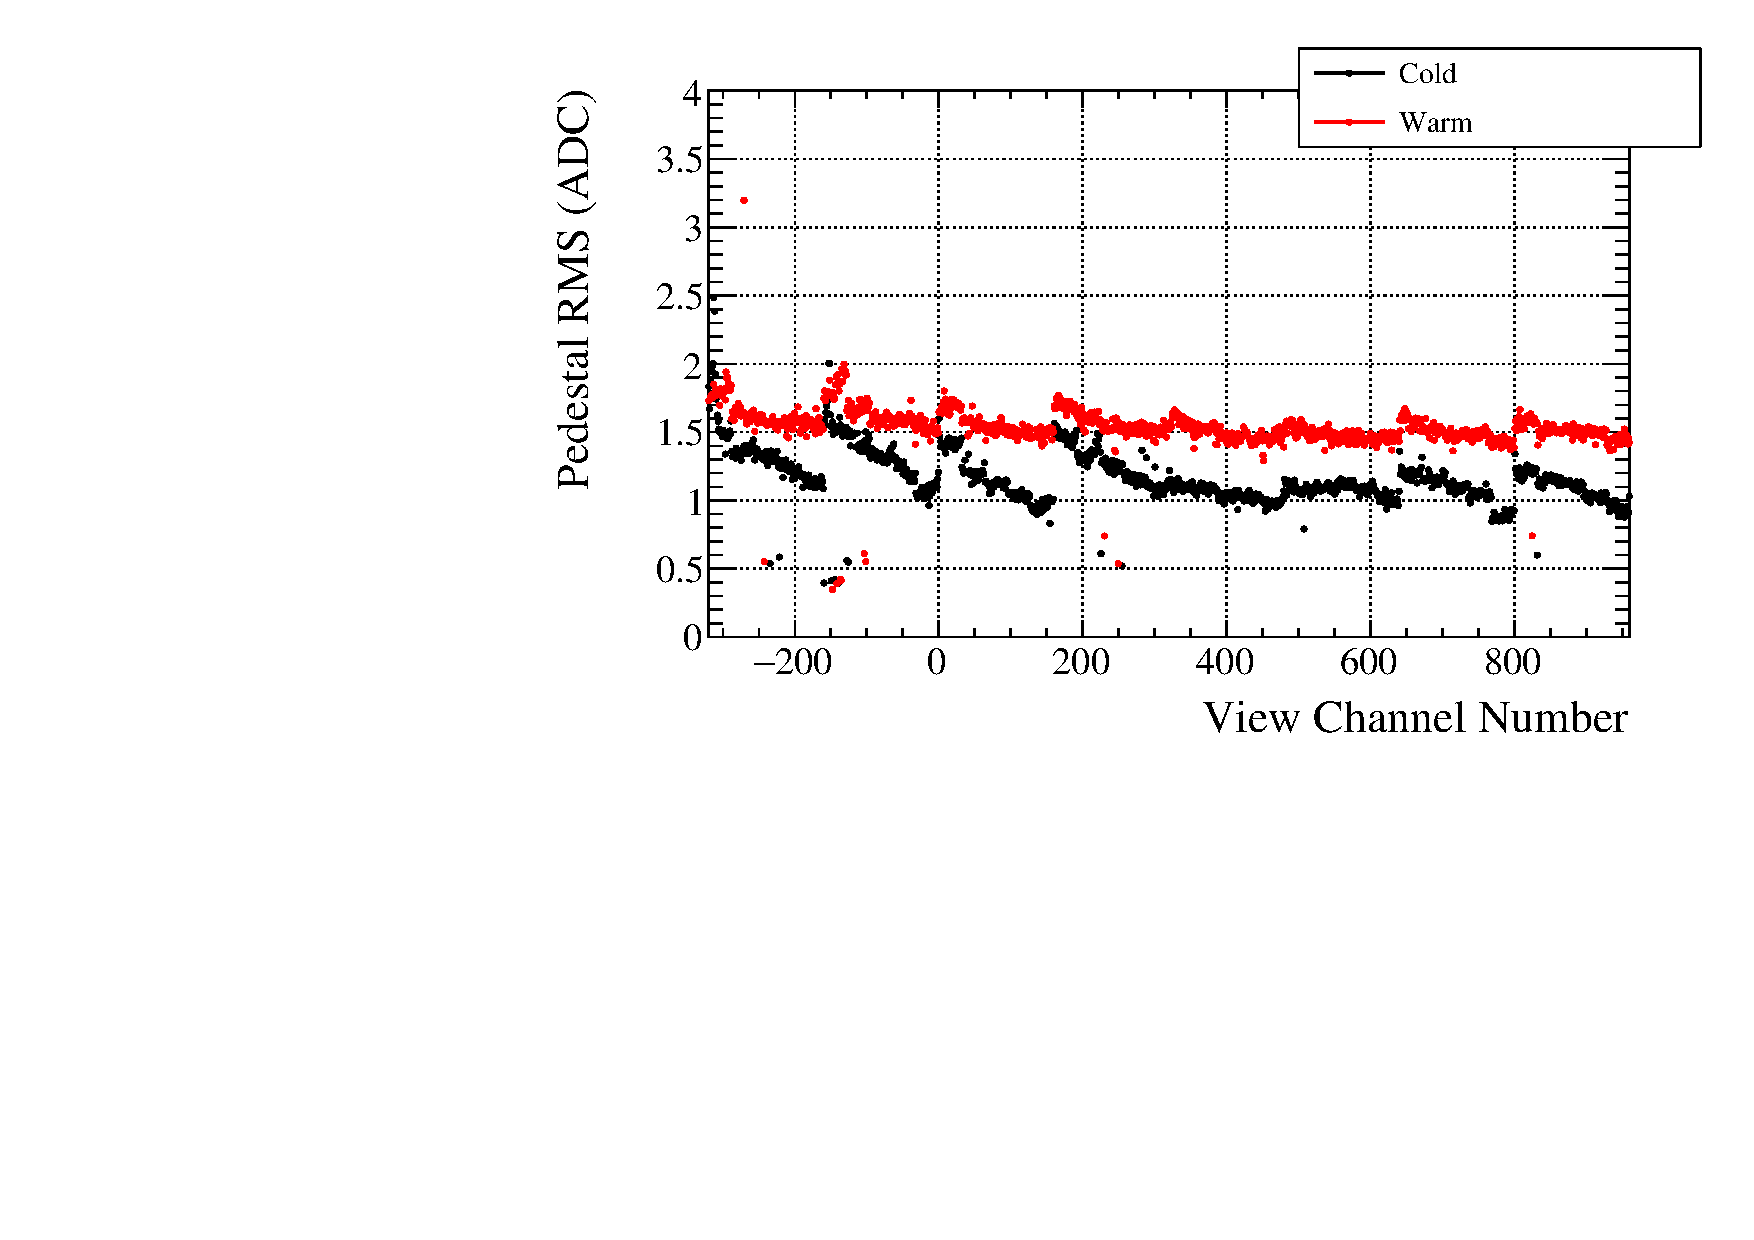
\includegraphics[width=0.45\textwidth]{dpele-311-noise-warm-cold}
\end{dunefigure}

While the \dword{fe} amplifier ASICs are in the shielded environment provided by the chimneys (Faraday cage), interference from other equipment via a noisy ground or ground loops could significantly worsen the noise performance from the design target. Figure~\ref{fig:dpele-311-noise} shows some results of the noise measurements performed under different conditions in the \dword{wa105} detector. The channels reading \SI{3}{\meter} (\SI{1}{\metre}) long strip correspond to negative (positive) channel numbering in the plots and the 1 \dword{adc} count is equivalent to about 900 electrons. The left plot of Figure~\ref{fig:dpele-311-noise} shows the noise measurements performed at warm with and without slow control cables (\dword{crp} HV, \dword{crp} motors, level meters, temperature probes, etc.) connected. The noise is clearly affected by the grounding of the slow control: the average value of the noise RMS is around \num{1.7} \dword{adc} with slow control cables connected and decreases to about \num{1.5} \dword{adc} when those are removed. As explained later, the grounding scheme of \dword{wa105} did not correspond to the one foreseen for DUNE, where all electrical equipment are referred uniquely to the cryostat ground and are completely insulated from the external environment. 

One interesting feature, particularly visible with the cables disconnected, is that the noise measured in \dword{wa105} is similar for the channels connected to the \SI{1}{\meter} and \SI{3}{\meter} long strips. Given that the longer strips have thrice the input capacitance than the shorter ones, the expected noise (see Figure~\ref{fig:dpele-fe-asic-prop}) for these should be larger by a about factor of two as indicated with the dashed line in the plot. In addition, the noise on the short strips is also lower (\num{1.5} \dword{adc}) than expected for the \SI{160}{pF/m} strip input capacitance (1.7 \dword{adc}). The reason for such behaviour of the noise in the \dword{crp} of \dword{wa105} is still under investigation. However, measurements have shown that the capacitance of the \dword{crp} anode strips is not purely to ground, but rather it is driven by the inter-strip couplings, which creates a more complicated electrical network. 

Figure~\ref{fig:dpele-311-noise} (right) also shows a comparison of the noise measurements in \dword{wa105} taken with the \dword{fe} electronics at warm (red points) and cold (black points) at around \SI{150}{\kelvin}. The slow control cables were disconnected in both cases. However, the measurements at cold were performed with the re-circulation pump active and the cathode HV connection present. The RMS noise averaged over all channels decreases by about 25\% from roughly \SI{1.5}{\dword{adc}} to \SI{1.1}{\dword{adc}} when the \dword{fe} analog cards are at cold. For comparison, the expected signal for a \dword{mip} with the \dword{crp} gain of 20 should be around \SI{200}{\dword{adc}}. 

The overall grounding principle of \dword{wa105} was based on having the cryostat as the ground reference. The low voltage power supplies for the \dword{fe} analog electronics and uTCA crates were powered via insulating transformers ensuring that they could see no other ground. On the other hand, the design of the slow control system did not include any insulation transformers. This equipment was grounded to the building electrical network thereby creating an interference with the ground of the cryostat. Stricter treatment of the ground connections, as foreseen for \dword{pddp} and the detector module, and a lower \dword{sft} chimney operating temperature of around \SI{110}{\kelvin} (from \SI{150}{\kelvin}) should help to reduce further the noise levels from those observed in \dword{wa105}.


%%%%%%%%%%%%%%%%%%%%%%%%%%%%%%%%%%%
\subsection{\dword{sft} Chimneys}
\label{sec:fddp-tpc-elec-design-sft}

The \dword{sft} chimneys are designed to enable the access to the \dword{fe} analog electronics for a potential repair or exchange while the detector is in operation (filled with the liquid argon). In addition, their metallic structure acts as a Faraday cage isolating the \dword{fe} ASICs from environmental interference.  Each \dword{sft} hosts \num{10} analog cryogenic \dword{fe} cards (reading \num{640} channels in total).  Some of the details of the design are illustrated in Figure~\ref{fig:dpele-sft-chimney-design}. 

\begin{dunefigure}[Details of the \dword{sft} chimney design]{fig:dpele-sft-chimney-design}
{Details of the \dword{sft} chimney design.}
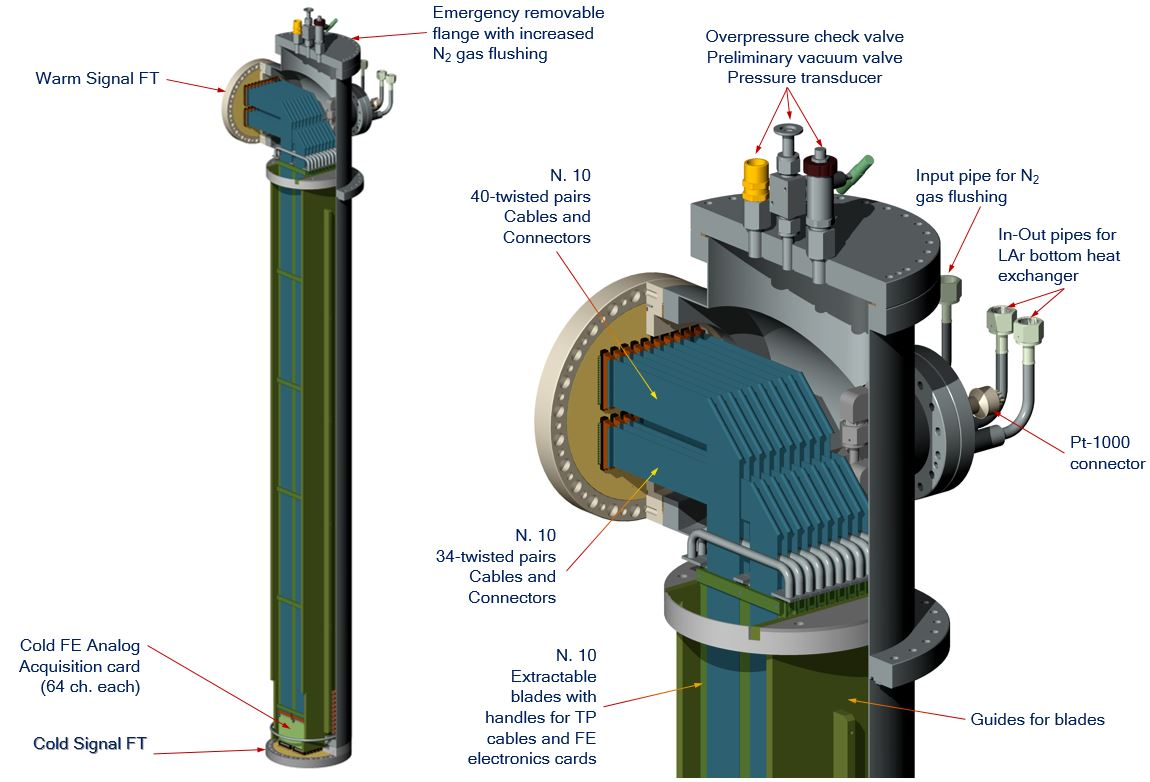
\includegraphics[width=0.8\textwidth]{dpele-sft-chimney-design}
\end{dunefigure}

The chimneys are closed at the bottom and top with vacuum tight feedthrough flanges whose function is to dispatch the signal and slow control lines. The feedthrough at the bottom, the cold (signal) feedthrough, isolates (Ulta-High Vacuum tightness standard) the inner volume of the detector module from the chimney volume and interconnects the signals from the \dword{crp} to the analog \dword{fe} cards. The feedthrough at the top, the warm (signal) feedthrough, seals the chimney from the outside environment. It also passes the low voltage and control lines to the \dword{fe} electronics inside and brings out the differential analog signal lines from the \dword{fe} amplifiers. 

The \dword{sft} chimney volume is filled with nitrogen gas at near atmospheric pressure. The temperature inside the chimney can be adjusted using a heat exchanger copper coil cooled with liquid argon. It is located at the bottom close to the cold feedthrough around the \dword{fe} cards. The functions of this cooling system are to mitigate the heat input to the main detector volume and provide optimal (lowest noise) operating temperature for the \dword{fe} electronics of around \SI{110}{K}. A pressure release valve, indicated in Figure~\ref{fig:dpele-sft-chimney-design}, protects the structure from an accidental overpressure in the inner volume. 

The expected heat input from a given \dword{sft} chimney is about \SI{20}{\watt}. This number includes the heat through the twisted-pair cables connected to the warm feedthrough, the \dword{sft} outer metallic tube, as well as the heat dissipation by the \dword{fe} cards. A total heat input from all \num{240} \dword{sft} chimneys is at the level of \SI{5}{\kilo\watt}. 

\begin{dunefigure}[\dword{sft} chimney cold flange]{fig:dpele-sft-cold-pcb}
{\dword{sft} chimney cold feedthrough flange with one of the \dword{fe} cards mounted.}
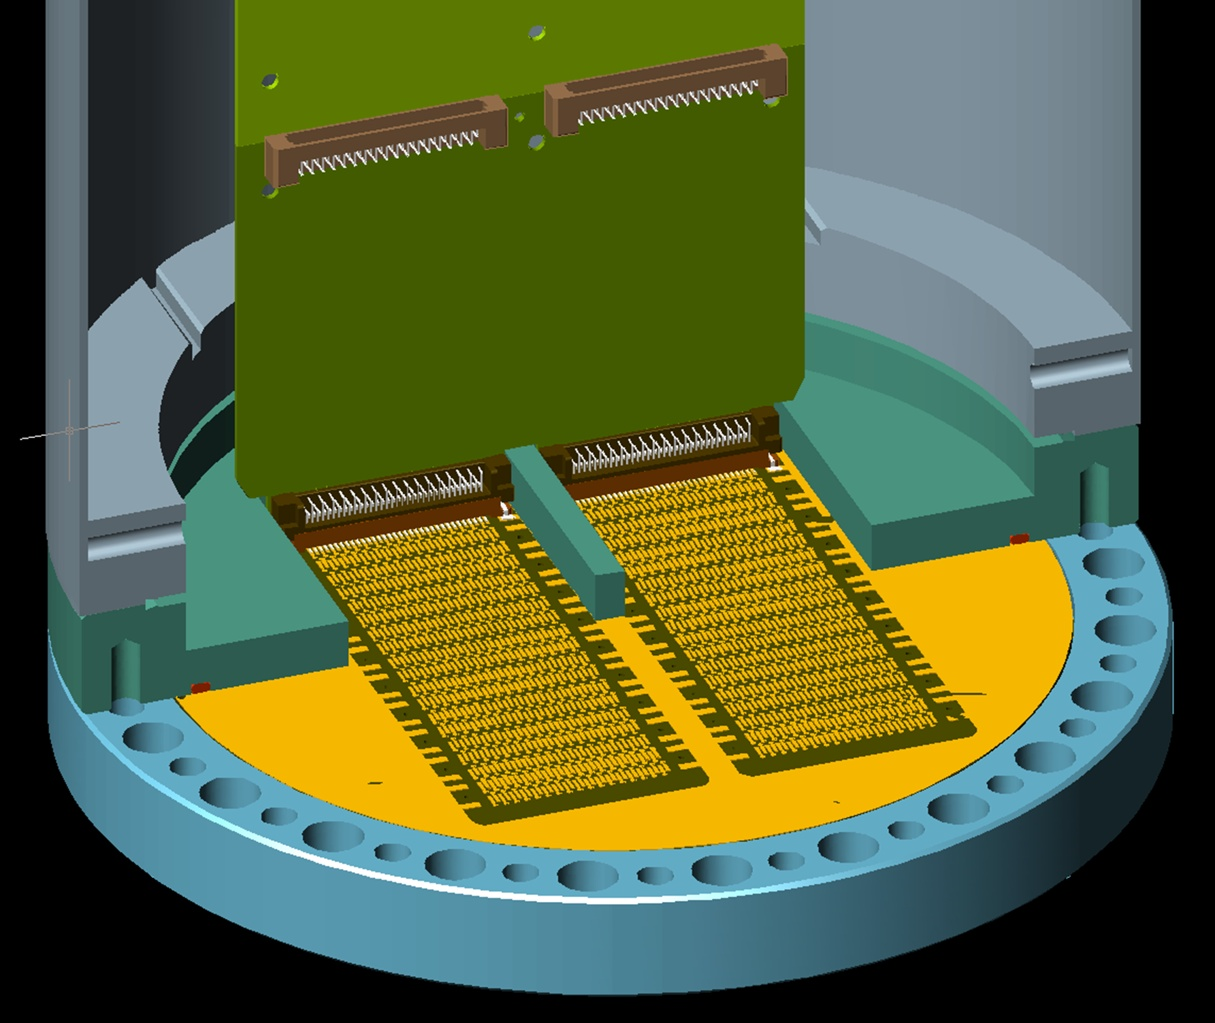
\includegraphics[width=0.6\textwidth]{dpele-sft-cold-pcb}
\end{dunefigure}

The analog \dword{fe} cards are inserted directly onto the PCB of the cold feedthrouh (see Figure~\ref{fig:dpele-sft-cold-pcb}). The other side of the PCB (facing inside the cryostat) hosts the connectors for the flat cables coming from the \dword{crp} anodes.  The \dword{fe} cards are mounted on \SI{2}{m} long blades made from FR4, which enable the insertion/extraction of the electronics and also support the flat cables carrying signals, low voltages, and slow control to/from the warm flange interface.  The blades slide along the rails installed inside the chimney at opposite sides, which guide the \dword{fe} cards to their respective connectors on the cold feedthrough. 

Prior to the commissioning of a detector module, the chimneys are evacuated via a dedicated KF16 port (see Figure~\ref{fig:dpele-sft-chimney-design}) and then filled with nitrogen gas. This ensures the removal of the moisture that would otherwise condense, once the detector module is filled with the liquid argon, around the \dword{fe} cards damaging the electronics. To access the \dword{fe} cards once the detector module is cold, the stainless steel flange at the top of the \dword{sft} chimney (Figure~\ref{fig:dpele-sft-chimney-design}) must be removed. This procedure requires continuous flushing of nitrogen gas at slight over-pressure with respect to the atmospheric in order to prevent the humid air entering and generating condensation inside the chimney. Once a chimney is opened, the blades with the \dword{fe} cards can be extracted after unplugging the flat cables (two per card) connected on the inner side of the warm flange (Figure~\ref{fig:dpele-sft-chimney-design}).

The procedure to access the \dword{fe} cards at cold was successfully tested during the operation of the \dword{wa105} detector. The temperature at the top of the chimney was very close to the room temperature allowing to manipulate the cable connections on the warm feedthrough flange without any cryogenic gloves. The movement of the blades on the rails and the \dword{fe} card extraction / insertion did not indicate any mechanical problems that could have been caused by shrinking of various elements due to the lower temperatures.  The signals from the \dword{fe} cards that underwent the extraction/insertion were also checked and no malfunctioning channels were found.

%%%%%%%%%%%%%%%%%%%%%%%%%%%%%%%%%%%
%\subsection{Low-voltage Power Supplies for \dword{fe} Electronics}
%\label{sec:fddp-tpc-elec-design-lvps}

%%%%%%%%%%%%%%%%%%%%%%%%%%%%%%%%%%%
\subsection{Digital AMC Electronics for Charge Readout}
\label{sec:fddp-tpc-elec-design-amc}
%THIS IS CHARGE READ OUT
The function of the \dword{cro} AMC cards is to read and digitize the data from the \dword{fe} amplifiers and then transmit them to the \dword{daq} system. The cards also include a last stage of analog shaping before the \dword{adc} input. The analog FEs produce differential unipolar signals defined with respect to a baseline offset. This offset is removed and the signals are subtracted in the analog input stage of the digital electronics prior to the digitization. Each card has eight \dword{adc} chips (AD9257, Table~\ref{tab:dpele-adc9257}), two dual-port memories (IDT70T3339), and an FPGA (ALTERA Cyclone V) on board. The FPGA provides a virtual processor (NIOS) that handles the readout and the data transmission. The choices for all of the components have been optimized with respect to the design requirements and technical criteria such as costs, chip footprint (small enough to fit on the AMC), power consumption, and ease of use (available functionality). 

\begin{dunetable}
[Main characteristics of \dword{adc} AD9257]
{lr} {tab:dpele-adc9257}
{Main characteristics of \dword{adc} AD9257.}
Item &   \\ \toprowrule
Channels & \num{8} \\ \colhline
Sampling & up to \SI{40}{MSPS} \\ \colhline %/\SI{65}{MSPS}
Resolution & \SI{0.122}{\milli\volt} \\ \colhline
Dynamic range & \num{14} bit/ \SI{2.0}{\volt} \\ \colhline
Differential Non-Linearity & Typical \num{\pm0.6} LSB\\ 
& with Min. \num{-1.0} and Max. \num{+1.7} LSB  \\ \colhline
Integral Non-Linearity & Typical \num{\pm1.1}  LSB\\
& with Min. \num{-3.1} and Max. \num{+3.1} LSB  \\ \colhline
\end{dunetable}


\begin{dunefigure}[Block diagram of AMC]{fig:dpele-amc-scheme}
{Block diagram of AMC.}
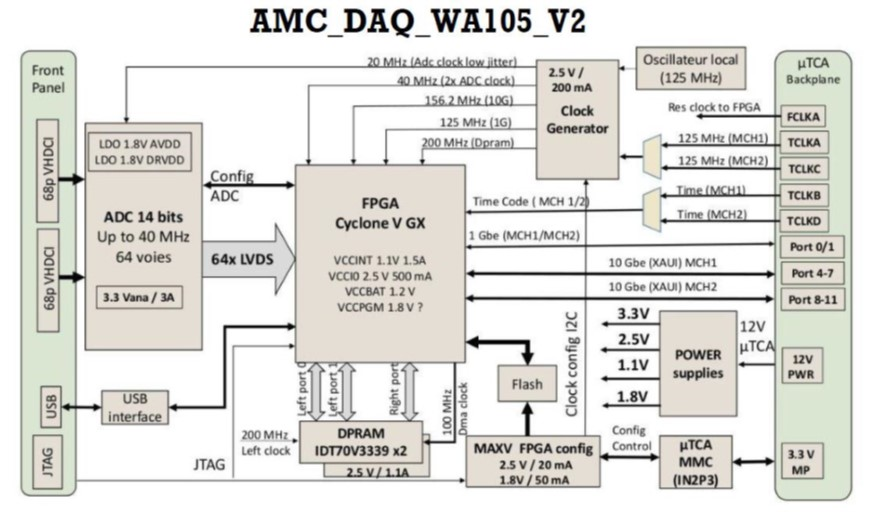
\includegraphics[width=0.9\textwidth]{dpele-amc-scheme}
\end{dunefigure}
Figure~\ref{fig:dpele-amc-scheme} shows block diagram of the AMC functionality. Each AMC generates a continuous compressed stream of \SI{2.5}{MSPS} 12 bit data per readout channel. The on-board ADCs operate at a rate of \SI{25}{\MHz} per channel. The data are down-sampled in the FPGA to \SI{2.5}{\MHz} by performing ten-sample averaging, which leads to the further digital filtering of the noise. The data, consisting of only \num{12} most significant bits from each digitized 14 bit sample, are then compressed using an optimized version of the Huffman algorithm and organized in frames for transmission.  The frames contain the absolute timing information of the first data sample for reliability purposes. In the current design, each AMC has 64 channels and reads one analog \dword{fe} card.

The AMCs are housed in uTCA crates and send their data via the MCH switch. The timing synchronization of AMCs is achieved via a WR-MCH module (also housed in the crate) that is connected to the White Rabbit network. In addition, WR-MCH could also be used for triggered readout of AMCs by sending it dedicated packets containing trigger timestamp information over the White Rabbit network.

In \dword{pddp}, AMCs are operated in the triggered mode reading \SI{4}{\milli\second} drift time window at trigger rate of \SI{100}{Hz}, which is not far from a continuous readout mode. The analog data are continuously digitized and buffered. A sub-sample of these data can then be acquired by providing AMC with a timestamp generated by an external trigger. The timestamp defines the start time for the data sequence to be read, while the length of the sequence is determined by the size of the drift window. In \dword{pddp} this length corresponds to \num{10000} (\SI{4}{\milli\second}) samples per full drift window.  Triggers (beam counters, cosmic ray counters, photomultipliers reading the UV light, starts of beam spills) are time stamped in a dedicated White Rabbit slave node (WR-TSN), an FMC-DIO mezzanine mounted on WR SPEC carrier card, which runs a custom firmware and is hosted in a computer. The WR-TSN is connected to the WR Grand Master for synchronization and for transmission of the trigger information. The timestamp data produced by the WR-TSN are sent over the White Rabbit network as Ethernet packets with a customized protocol. 

%%%%%%%%%%%%%%%%%%%%%%%%%%%%%%%%%%%
\subsection{Electronics for Light Readout}
\label{sec:fddp-tpc-elec-design-lro}

%
The LRO card is a \num{16} channel AMC containing one \num{16} channel \num{14} bit \SI{65}{\MHz} \dword{adc} (AD9249) and one \dword{catiroc} ASIC \cite{Blin:2017}. A block diagram of the prototype board used for \dword{pddp} is shown in Figure~\ref{fig:dpele-lro-scheme}. In this prototype, Figure~\ref{fig:dpele-lro-proto}, a mezzanine board containing the ASIC and \dword{adc} sits on a commercial (COTS) mother board (Bittware S4 AMC) with a high specification FPGA (ALTERA Stratix IV). In the final implementation for the DUNE, the mezzanine is integrated with the layout of the AMC board developed for the charge readout.  
A proposed upgrade is a \num{32} channel card, diminishing the number of cards required and increasing the channel density to \num{352} channels per uTCA crate.

\begin{dunefigure}[Block diagram of LRO]{fig:dpele-lro-scheme}
{Block diagram of LRO prototype.}
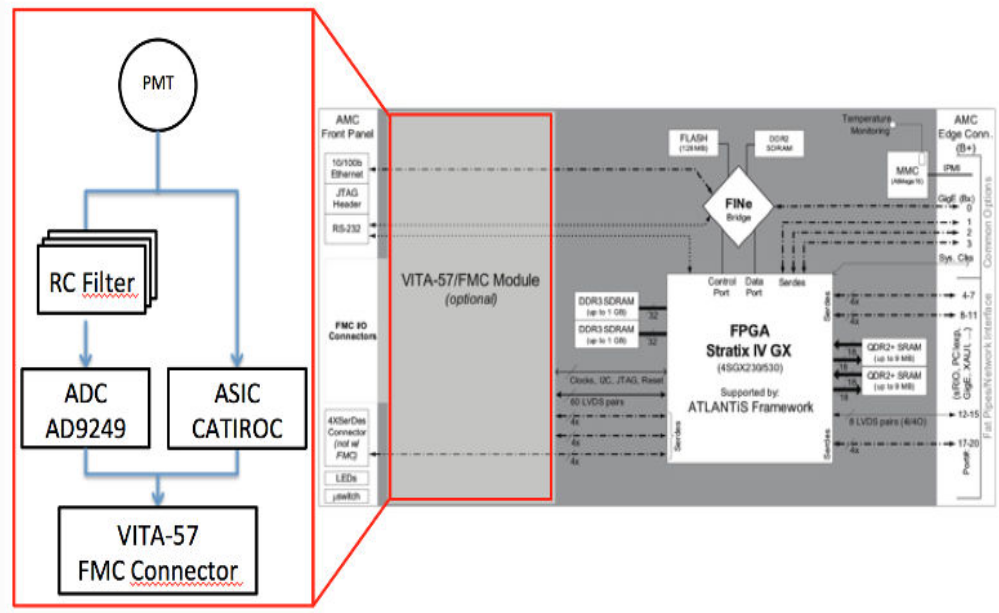
\includegraphics[width=0.7\textwidth]{dpele-lro-scheme}
\end{dunefigure}

\begin{dunefigure}[Prototype LRO card]{fig:dpele-lro-proto}
{The LRO prototype.}
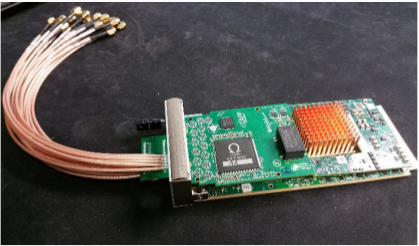
\includegraphics[width=0.7\textwidth]{dpele-lro-proto}
\end{dunefigure}

The analog signals from each \dword{pmt} channel are split equally into two separate branches (see Figure~\ref{fig:dpele-lro-scheme}) . One path (Waveform branch), through an anti-aliasing low-pass filter and the \num{14} bit \SI{65}{\MHz} \dword{adc} (AD9249), produces continuous digitization of the \dword{pmt} waveform data, which are down-sampled to \SI{2.5}{MHz} prior to the transmission to \dword{daq}. The other (\dword{catiroc} branch) is routed directly to the \dword{catiroc} ASIC for precise measurements of pulse charge and timing. Both paths produce data continuously and independently.


\subsubsection{Waveform branch} %\dword{adc}
%details on \dword{catiroc}
The main characteristics of the \dword{adc} used for continuous digitization of the \dword{pmt} signals are shown in Table \ref{tab:dpele-adc9249}.
%RMS and \dword{pmt} gain?
\begin{dunetable}
[Main characteristics of \dword{adc} AD9249]
{lr} {tab:dpele-adc9249}
{Main characteristics of \dword{adc} AD9249.}
Item &   \\ \toprowrule
Channels & \num{16} \\ \colhline
Sampling & \SI{65}{MSPS} \\ \colhline
Resolution & \SI{0.122}{\milli\volt} \\ \colhline
Dynamic range & \num{14} bit/ \SI{2}{\volt} \\ \colhline
Differential Non-Linearity & Typical \num{\pm0.6} LSB\\
& with Min. \num{-0.9} and Max. \num{+1.6} LSB  \\ \colhline
Integral Non-Linearity & Typical \num{\pm0.9}  LSB\\
& with Min. \num{-3} and Max. \num{+3} LSB  \\ \colhline
%MEMORY??
\end{dunetable}
%noise llevel??

For normal operation, in continuous sampling mode, the time samples are down-sampled by the FPGA to a coarse \SI{400}{ns} sampling to match that of the Charge Read Out and limit the quantity of data streamed. The use of a higher specification \dword{adc}, with time-sampling of \SI{15.4}{ns}, allows for greater flexibility.  It is envisaged that for particular calibration runs, waveforms with finer time-sampling could be read-out which would allow studies of, for example, the liquid argon scintillation time-profiles. Even in normal operation, online pulse processing is possible within the FPGA using the finer time-sampled waveforms (before the down-sampling), which could be used to make continuous measurements such as the rise and fall times of the pulses. Even at the coarse sampling of \SI{400}{ns} studies of the liquid argon scintillation time-profile are possible (with the long fall timeconstant of $\sim$\SI{1500}{ns}) and also matching of the electroluminescence signal (also known as proportional scintillation light) to that of the charge signal.  Low light-level signals, such as the single or few photoelectron signals, will show no time structure, but will consist of 1 sample several LSB above the baseline. 

\subsubsection{CATIROC branch} %{Analog Measurements of Charge and Time}%ASIC?

The \dword{catiroc} is a \num{16} channel ASIC dedicated to measurement of charge, and precision timing of negative-polarity \dword{pmt} signals \cite{Blin:2017}. It auto-triggers on single photo-electrons, and can sustain a high dark rate of up to \SI{20} {kHz/channel}. Charge measurements can be made over the range of \SI{160}{fC} to \SI{70}{pC} (corresponding to approximately to a range of \num{1} - \num{400} photo-electrons with a \dword{pmt} gain of \num{1E6}). Timing measurements per channel can be made with an accuracy of \SI{200}{ps}.

\begin{dunefigure}[\dword{catiroc} ASIC]{fig:dpele-lro-catiroc}
{Functional diagram of \dword{catiroc} ASIC.}
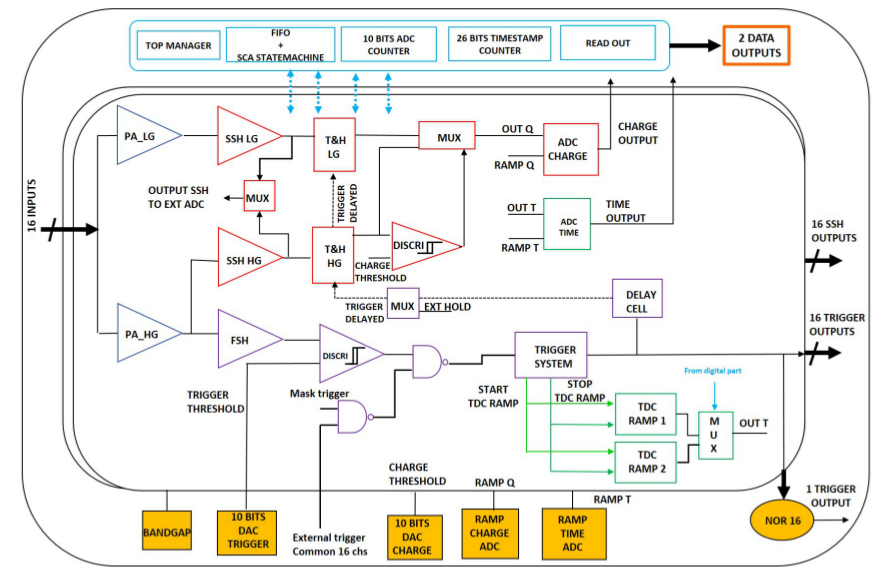
\includegraphics[width=0.7\textwidth]{dpele-lro-catiroc}
\end{dunefigure}

Figure~\ref{fig:dpele-lro-catiroc} shows the schematic of the \dword{catiroc} ASIC. Its main properties are summarized in Table~\ref{tab:dpele-catiroc}. The slow channel, from which precision charge and timing measurements are made, is formed by two variable gain (\SI{8}{bit}) amplifiers followed by two variable slow shapers; one High Gain for small signals, and one Low Gain for larger signals, and two Track-and-Hold stages. The slow shaper has a tunable shaping time (up to \SI{100}{ns}) and a variable gain.  If the High Gain is saturated, corresponding to passing a pre-determined threshold common to all 16 channels, the Lower Gain value is chosen. The chosen charge value is converted by an internal 10-bit Wilkinson \dword{adc} operating at \SI{160}{MHz}.  This slow channel operates in a ping-pong mode, with two capacitors to store the slow shaper signals, giving an effective buffer of 2 events. If both capacitors are full, a deadtime of \SI{5}{\micro\second} arises.

\begin{dunetable}
[Main characteristics of \dword{catiroc}.]
{lr} {tab:dpele-catiroc}
{Main characteristics of \dword{catiroc}.}
Item &   \\ \toprowrule
Number of channels & \num{16}\\ \colhline
Signal polarity & negative \\ \colhline
Timing & Timestamp: 26 bit counter at \SI{40}{MHz} \\
       & Fine time: resolution $<$\SI{200}{ps}\\ \colhline
Charge Dynamic Range & \SI{160}{\femto\coulomb} to \SI{100}{\pico\coulomb}\\ \colhline
Trigger & auto-trigger \\
        & Noise = \SI{5}{fC} Minimum threshold = \SI{25}{fC} (5$\sigma$)\\ \colhline
Digital & 10-bit Wilkinson \dword{adc} at 160 MHz \\ %TWO READOUT AT 80MHZ??
        & Read-out frame of 50 bits \\ \colhline
Outputs & \num{16} trigger outputs \\
        & NOR16 \\
        & \num{16} slow shaper outputs \\
        & Charge measurement over \num{10} bits \\
        & Time measurements over \num{10} bits \\ \colhline
Main Internal &  Variable preamplifier gain \\
Programmable  &  Variable shaping and gain \\
Features & Common trigger threshold \\
         & Common gain threshold \\ \colhline
\end{dunetable}

The fast channel is used to auto-trigger the ASIC and make the fine-timing measurement. It comprises a high gain preamplifier, fast shaper (shaping time \SI{5}{ns}) and discriminator with a \num{10} bit programmable threshold that is common to all \num{16} channels. The output of the discriminator is used for the two Time to Digital Convertors to get the fine-timing. A coarse timestamp could also be obtained from a \num{26} bit counter running at \SI{40}{MHz}.  Only the data from the triggered channels are digitized; their information is transferred to the internal memory, which is read by the external FPGA. 

  
%%%%%%%%%%%%%%%%%%%%%%%%%%%%%%%%%%%
\subsection{Network-based uTCA Architecture}
\label{sec:fddp-tpc-elec-design-utca}

The digital electronics is based on uTCA standard which offers industrial solution with a very compact and easily scalable architecture to handle a large number of channels at low cost.  The standard (or related standards such as ATCA or xTCA) is widely used in the telecommunication industry and is being adapted by the HEP community. The backplane of the uTCA crates host high-speed serial links that support a variety of transmission protocols (Ethernet, PCI Express, SRIO, etc.). In addition, dedicated lanes are available for the distribution of the clock signals to all the boards hosted in the crate.  The Ethernet-based solution has been adopted for both the data and clock distribution in this design of the DP electronics system for both Charge and Light Read Out. 

Each AMC for either charge or light readout plugged into the uTCA is connected to the crate MCH board through the backplane serial links. The MCH provides the switch functionality that enables AMCs to communicate with each other or external systems through the MCH uplink interface. In the DP electronics system design, MCH also manages the WR clock distribution. 

\begin{dunetable}
[Bandwidth requirements per uTCA crate.]
{lr}{tab:dp-utcabandwidth}
{Bandwidth requirements per uTCA crate for continuous data streaming. A compression factor of 10 for the charger readout data is assumed }   
Parameter & Value  \\ \toprowrule
  \dword{cro} data rate  &  \SI{1.8}{Gibit/s}         \\ \colhline
  LRO data rate  &  \SI{4.7}{Gibit/s}            \\ \colhline
  Current MCH bandwidth & \SI{10}{Gibit/s}              \\ \colhline
  Upgradable MCH bandwidth & \SI{40}{Gibit/s}           \\ \colhline
\end{dunetable}

In the current design, as used for \dword{pddp}, the MCH operates with a \SI{10}{Gbit/s} uplink. Given that a uTCA crate hosts \num{10} AMCs for charge readout, the required bandwidth to stream the data to \dword{daq} is about \SI{1.8}{Gbit/s}. This assumes that the data exiting the AMCs are losslessly compressed with the compression factor of \num{10}. The bandwidth required per crate link for streaming the \dword{lro} data is \SI{4.7}{Gbit/s}. The \SI{10}{Gbit/s} MCH is therefore sufficient to support these data rates. However, the technology is moving towards supporting the \SI{40}{Gbit/s} rates. In addition, the channel density per AMC could also be increased for cost optimization. For these reasons an upgrade to a \SI{40}{Gbit/s} MCH could be foreseen in the future. This would also imply that the optical links connecting the \dword{daq} system to uTCA MCH should be operable at \SI{40}{Gbit/s}. A summary of the required and supported bandwidths per uTCA crate for continous data streaming is provided in Table~\ref{tab:dp-utcabandwidth}.

\begin{dunefigure}[Pictures of an instrumented uTCA crate from \dword{wa105} detector]{fig:dpele-311-utca-image}
{Pictures of an instrumented uTCA crate from \dword{wa105} detector. The crate contains five AMC cards, correspondingly to the number of readout channels per the \dword{sft} chimney. The images below show the crate after the  cables are connected to the warm flange of the \dword{sft} chimney.}
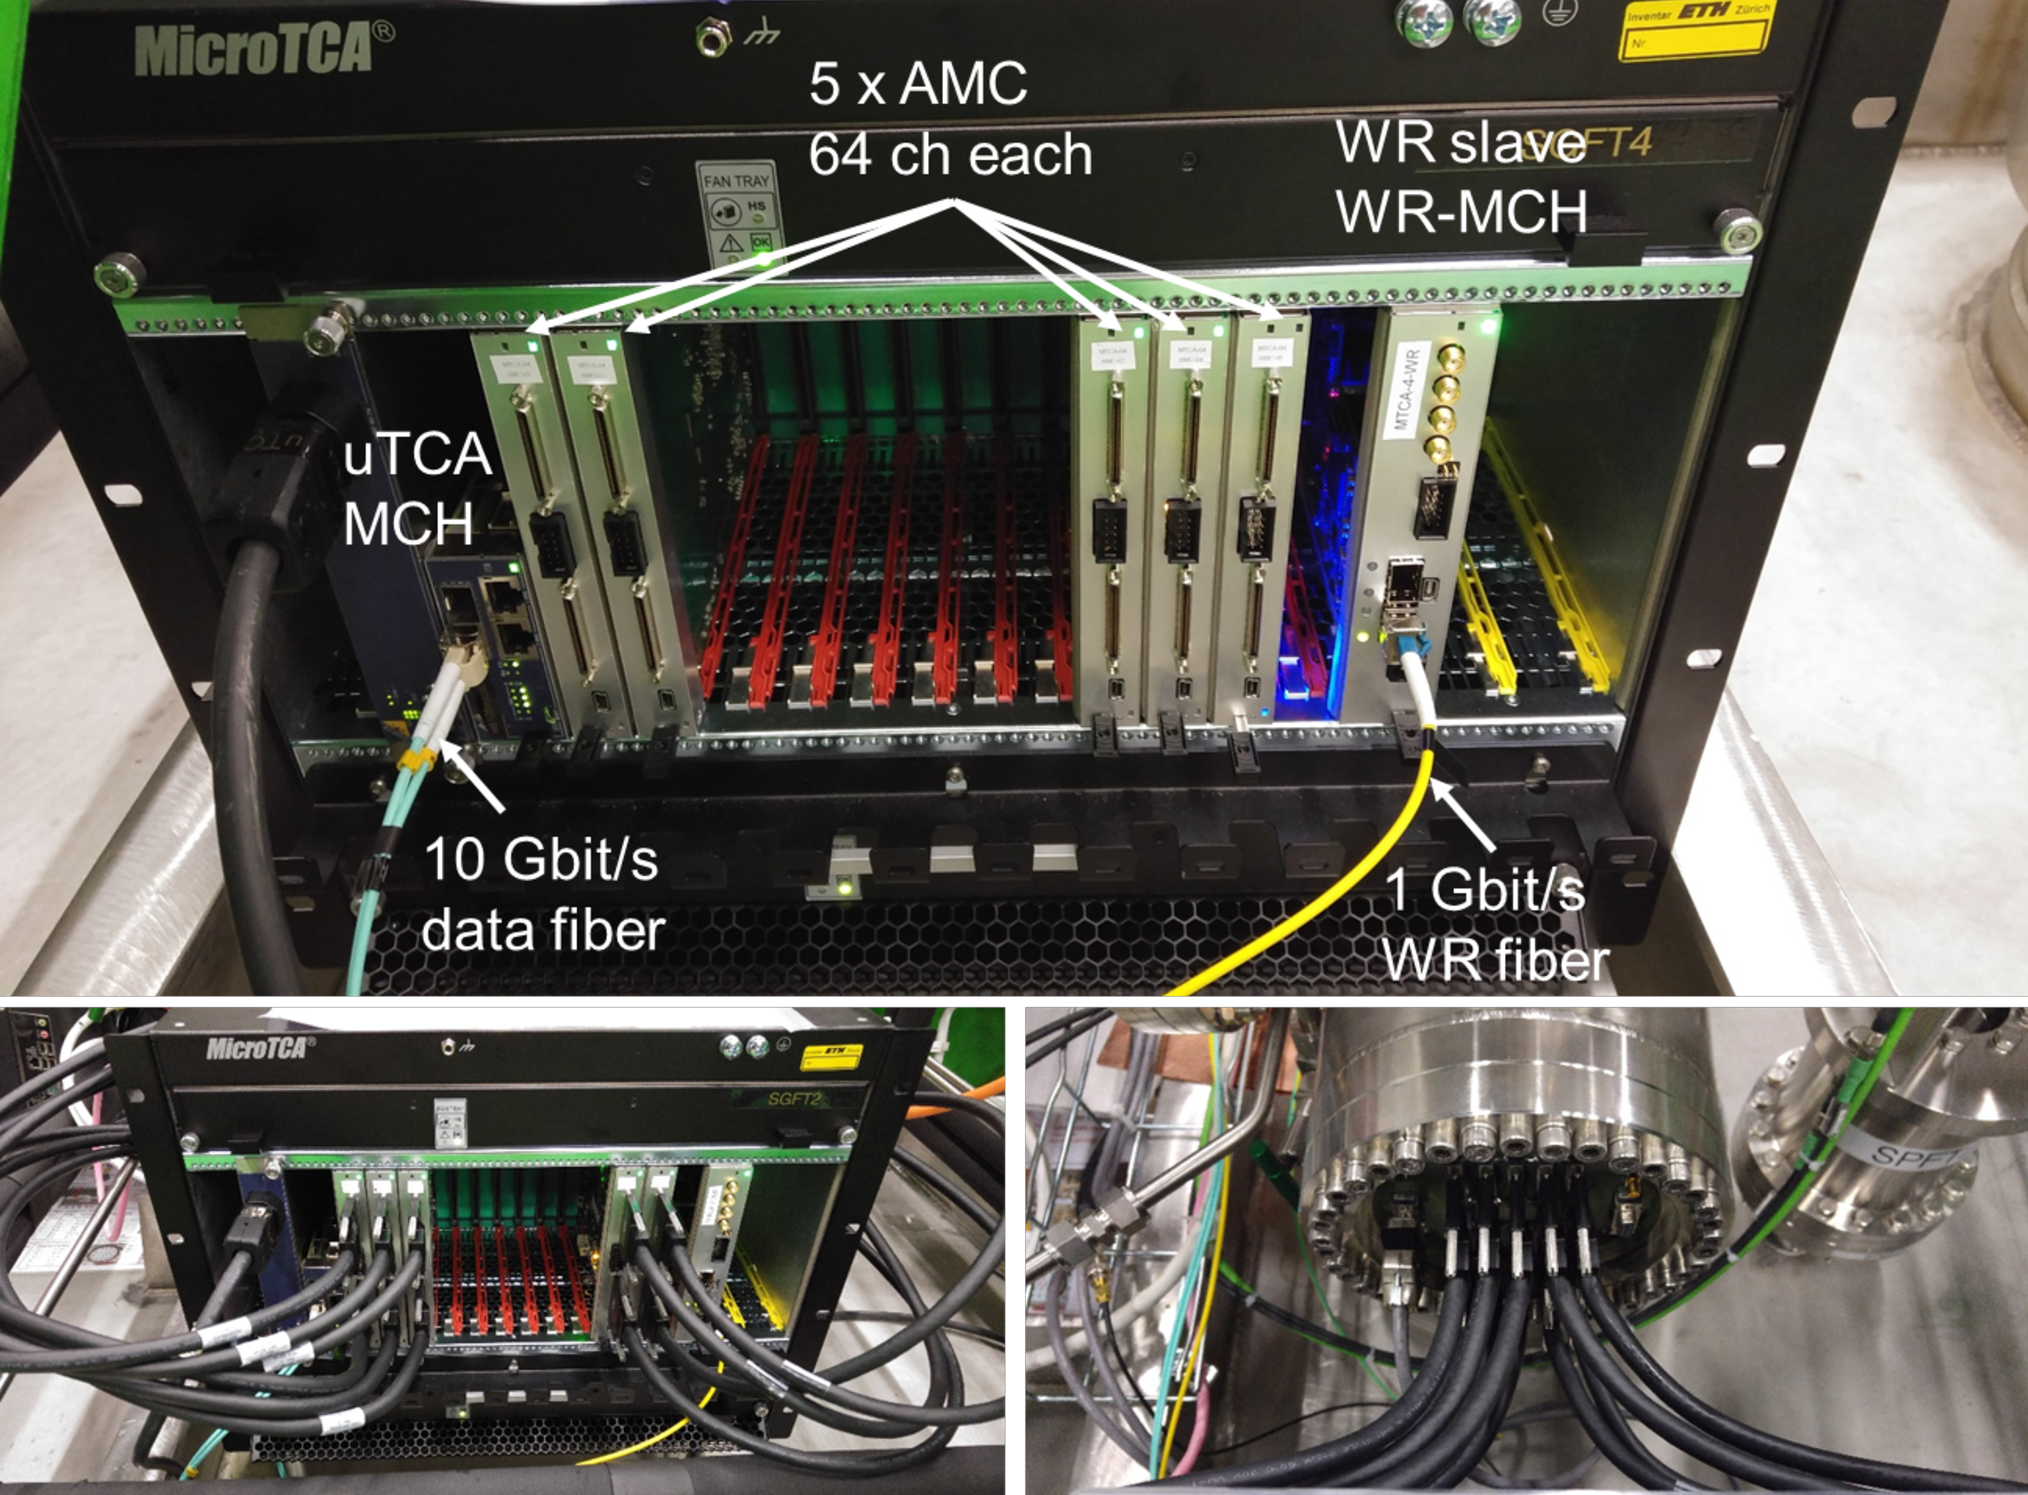
\includegraphics[width=0.6\textwidth]{dpele-311-utca-image}
\end{dunefigure}

As an illustration, Figure~\ref{fig:dpele-311-utca-image} shows pictures of one of the instrumented uTCA crates used for the charge readout of \dword{wa105} at CERN. In this detector each \dword{sft} chimney reads \num{320} channels thus requiring only five AMCs per the uTCA crate. The two optical fiber links, one (\SI{10}{Gbit/s}) for data and the other (\SI{1}{Gbit/s}) for clock/trigger timing distribution, are visible in the images.       

%%%%%%%%%%%%%%%%%%%%%%%%%%%%%%%%%%%
\subsection{Timing Distribution}
\label{sec:fddp-tpc-elec-wr}
% WR description and card development
The time synchronization system utilizes a White Rabbit (WR) network, which combines the synchronous \SI{1}{Gbit/s} Ethernet (SyncE) technology with the exchange of PTPV2 packets, to synchronize clocks of distant nodes to a common time. A high stability GPS disciplined oscillator (GPSDO) with the accuracy similar to that of an atomic clock provides a clock reference signal to be distributed over the physical layer interface of the WR Ethernet network. The network topology is built using specially designed switches that have the standard IEEE802.1x Ethernet Bridge functionality with an addition of WR-specific extensions to preserve the clock accuracy. Time and frequency information are distributed to the nodes on the WR network via optical fibers. The WR protocol automatically performs dynamic self-calibrations to account for any propagation delays and keeps all connected nodes continuously synchronized to sub-ns precision. 

The sub-ns accuracy on the clock synchronization is not strictly needed for aligning samples in the different AMC digitization units, since the data have the timing granularity of 400 ns. However, WR timing system offers readily available industrial components and necessary protocols needed for synchronization with automatic calibration of delay propagation and it, therefore, has been adopted. This solution for the timing distribution was part of the R\&D started in 2006 and the final design for integrating this system with the readout of the \dword{pddp} detector was completed in 2016.

In the implementation specific to \dword{pddp}, a GPS disciplined clock unit (Meinberg LANTIME M600) feeds 10 MHz and 1 PPS reference signals to a commercial White Rabbit switch (Seven Solutions WRS V3.4). The switch acts as Grand Master of the WR network. It is connected via 1Gbit/s optical links to the dedicated WR timestamping node (WR-TSN) and the WR end-node slave cards present within each uTCA crate (WR-MCH) keeping these synchronized to its reference time. The Grand Master also communicates through a standard Ethernet port with the LANTIME unit for its date and time synchronization via NTP. The WR-TSN module recieves analog TTL-level trigger signals, generates their timestamps, and then transmit these over WR network to the connected WR-MCH units. This timestamp information is then used by AMCs to find the data frame corresponding to the trigger. 

\begin{dunefigure}[Picture of White Rabbit slave WR-MCH card]{fig:dpele-wrmch-image}
{Picture of the WR slave node card (WR-MCH) present in each uTCA crate for time synchronization.The WR-LEN mezzanine card is visible in the bottom right corner.}
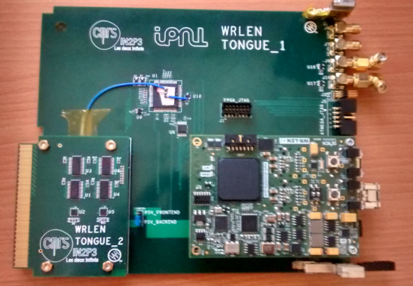
\includegraphics[width=0.45\textwidth]{dpele-wrmch-image}
\end{dunefigure}

The WR-MCH card (Figure~\ref{fig:dpele-wrmch-image}) enables clock/timing/trigger distribution to AMCs. It communicates with them via dedicated lines in the backplane of the uTCA crate using a customized data-frame protocol. The module contains a commercial WR slave node card, the White Rabbit Lite Embedded Node (Seven Solutions OEM WR-LEN), as mezzanine card. WR-LEN runs on a customized firmware which also enables it to decode the trigger timestamp data packet received over the WR network.

\begin{dunefigure}[Architecture of White Rabbit network]{fig:dpele-wrnet-layout}
{Architecture of WR network for time synchronization of digital readout electronics.}
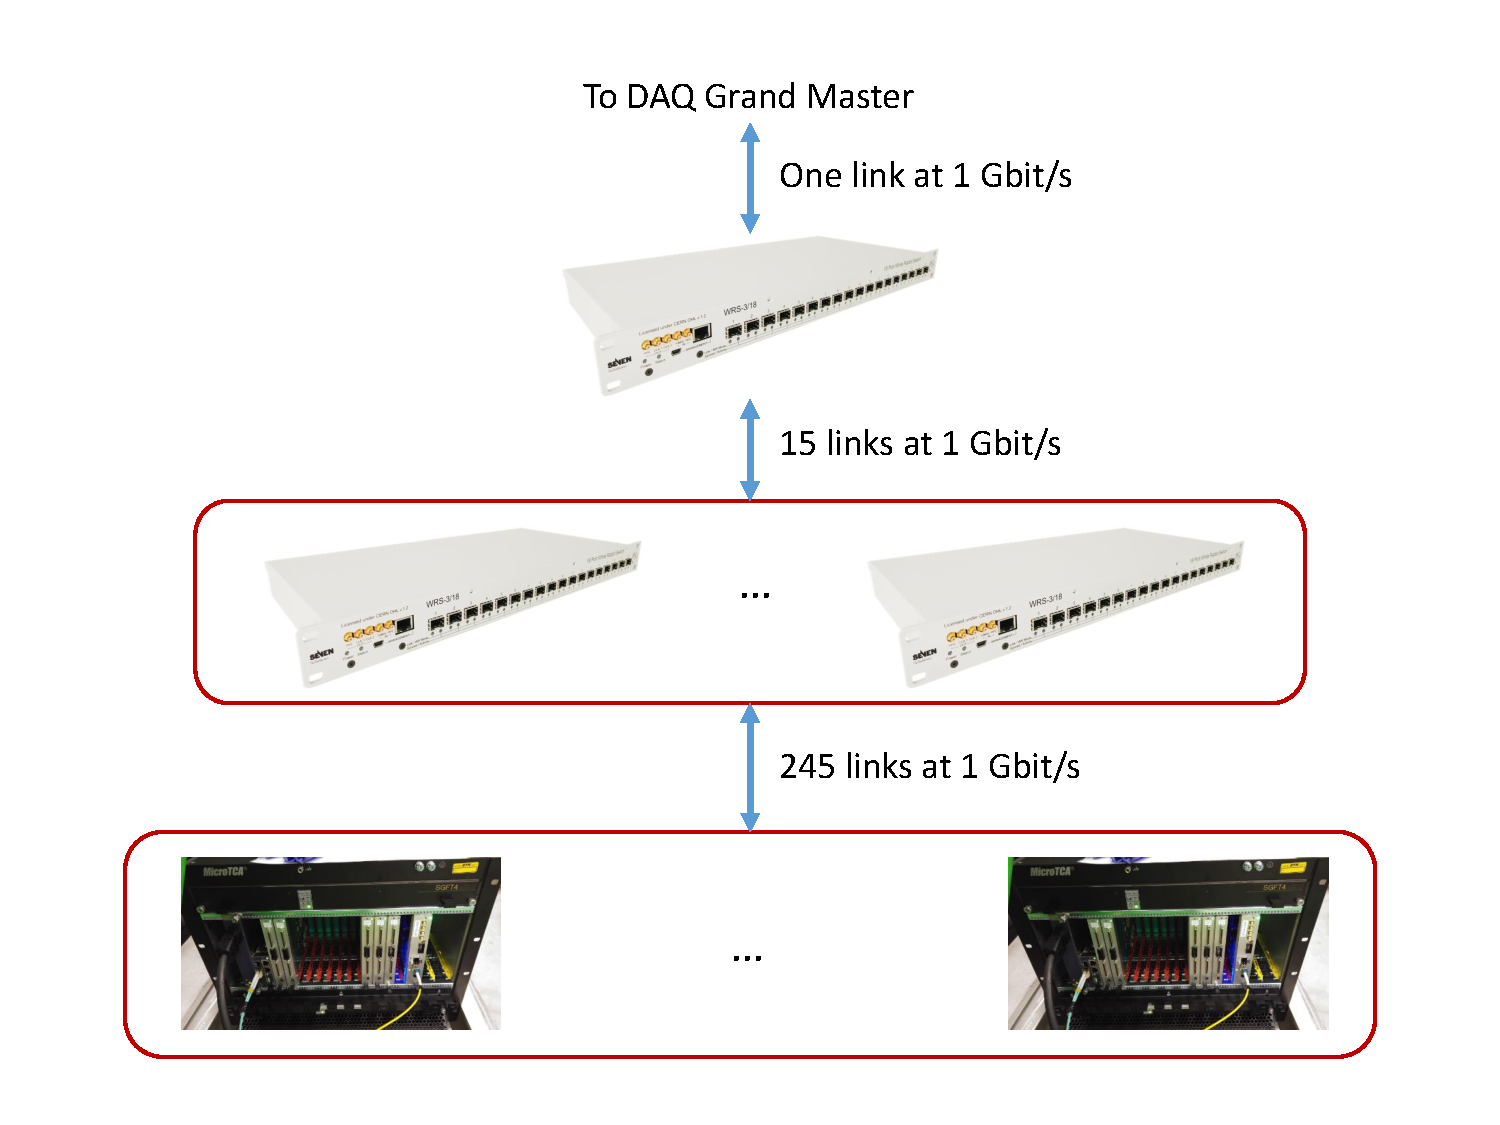
\includegraphics[width=0.7\textwidth]{dpele-wrnet-layout}
\end{dunefigure}

The architecture of the WR network layout for one DP detector module is illustrated Figure~\ref{fig:dpele-wrnet-layout}. It is built in a hierarchical structure from \num{16} WR switches with \num{18} ports each,  chained with \SI{1}{Gbit/s} optical fibers. The switch at the top of the hierarchy interconnects the synchronization Grand Master from the \dword{daq} system with the \num{15} switches in the middle layer. Those are in turn connected to the WR-MCH slave nodes in each uTCA crate (245 in total for charge and light readout). 



%%%%%%%%%%%%%%%%%%%%%%%%%%%%%%%%%%%%%%%%%%%%%%%%%%%%%%%%%%%%%%%%%%%%
\section{Production and Quality Assurance}
\label{sec:fddp-tpc-elec-prod-assy}

%%%%%%%%%%%%%%%%%%%%%%%%%%%%%%%%%%
\subsection{Cryogenic Analog \dword{fe} Electronics}
\label{sec:fddp-tpc-elec-prod-fe}
<<<<<<< Updated upstream
The production of the cryogenic ASICs and analog FE cards is envisioned to be split between several sites located in France and Japan at the moment. The delivered cards are then split between five institutions in France (IPNL), Japan (KEK, NITKC, IU), and USA (SMU), where they are tested for various performance parameters such as noise levels, dead channels, hot channels, gain and its uniformity across channels, etc., at both room and operating cold temperature. An appropriate and common database will be developed and populated with test results. 
=======
The production of the cryogenic ASICs and analog \dword{fe} cards is envisioned to be split between several sites located in France and Japan at the moment. The delivered cards are then split between between five institutions in France (IPNL), Japan (KEK, NITKC, IU), and USA (SMU), where they are tested for various performance parameters such as noise levels, dead channels, hot channels, gain and its uniformity across channels, etc., at both room and operating cold temperature. An appropriate and common database will be developed and populated with test results. 
>>>>>>> Stashed changes

%%%%%%%%%%%%%%%%%%%%%%%%%%%%%%%%%%
\subsection{\dword{sft} Chimneys}
\label{sec:fddp-tpc-elec-prod-sft}
The production of \dword{sft} chimneys consist of manufacturing of the PCB flanges for warm and cold feedthrough flange interfaces, the stainless steel pipe structure and the flanges containing the interfaces to the gas/liquid lines and slow control, the blades and railing, and the heat exchanger system. The flat cables that connect the \dword{fe} cards to the warm flange are commercially available products and are also procured at this stage.

The produced pieces are delivered to one or several institutions participating in the DP electronics consortium. The signal continuity is verified for both cold and warm flanges. The \dword{sft} chimneys are then assembled and tested for leaks. The blade insertion is also checked and the flat cables are tested. The assembled \dword{sft} chimneys are then packed and shipped to SURF. 

%%%%%%%%%%%%%%%%%%%%%%%%%%%%%%%%%%
\subsection{Timing System and uTCA}
\label{sec:fddp-tpc-elec-prod-utca}

The timing system consisting of \num{16} WR switches and the \num{245} uTCA crates containing the power modules, carrier hubs (MCH), and fan units are commercial components. The manufacturer takes the responsibility for the necessary quality control and assurance of these components requiring no further testing on the part of the DP electronics consortium. Once they are delivered to the designated institutions, they can be sent to SURF for the installation. 

The commerical VHDCI signal cables (connecting the AMCs to the \dword{sft} chimneys) are procured and tested with the \dword{sft} chimney warm flanges.

%%%%%%%%%%%%%%%%%%%%%%%%%%%%%%%%%%
%\subsection{Low-voltage Power Supply System}
%\label{sec:fddp-tpc-elec-prod-lvps}

%%%%%%%%%%%%%%%%%%%%%%%%%%%%%%%%%%%
%\subsection{Digital Electronics}
%\label{sec:fddp-tpc-elec-prod-amc}

\subsection{Charge Readout Electronics}
\label{sec:fddp-tpc-elec-prod-cro}
The production of the AMC cards for the charge readout as well as the WR-MCH slave cards for synchronization is currently shared between four institutions (IPNL, KEK, NITKC, IU). The cards ordered and delivered to each respective institution are subjected to quality assurance tests agreed upon by all participants.  

%%%%%%%%%%%%%%%%%%%%%%%%%%%%%%%%%%%
\subsection{Light Readout Electronics}
\label{sec:fddp-tpc-elec-prod-lro}

<<<<<<< Updated upstream
The production of the Light Read Out AMC cards is currently envisaged to be made in the same manner as the cards for \dword{pddp} since the number of cards to be produced, and channels to test, is small. The electronic components will be purchased, to required specifications, for the production of the card. The project will be managed by a qualified engineer, and followed by a specialist in Quality assurance.
=======
The production of the \dword{lro} AMC cards is currently envisaged to be made in the same manner as the cards for \dword{pddp} since the number of cards to be produced, and channels to test, is small. The electronic components will be purchased, to required specifications, for the production of the card. The project will be managed by a qualified engineer, and followed by a specialist in Quality assurance.
>>>>>>> Stashed changes

The produced cards are first delivered to the home institutes for testing before being shipped to the DUNE far site.  Basic quality tests are made upon delivery to ensure conformity of production; including visual inspection and electrical testing.

A series of tests are performed on each card to ensure their correct functionality and to evaluate their performance. Measurements include; linearity measurements (DNL and INL) of each \dword{adc} channel, and tests of the linearity of response of the ASIC. The level of cross-talk on the ASIC %must also be 
is also quantified.

A dedicated single channel setup, with \dword{pmt} (Hamamatsu R5912-02-mod), and identical cabling and splitter, can be used to characterise the expected noise level of each channel, and response to single photoelectrons up to saturation. 

Multiple cards are operated in a uTCA crate with the DUNE \dword{daq}.

After shipping and installation on-site, a small series of tests are performed with a pulse generator to verify the good working condition of the cards. Noise level measurements are also made as part of the integration effort.

%%%%%%%%%%%%%%%%%%%%%%%%%%%%%%%%%
%\subsection{Assembly Procedures}
%\label{sec:fddp-tpc-elec-assy}

%%%%%%%%%%%%%%%%%%%%%%%%%%%%%%%%%%%
%\subsection{Quality Assurance}
%\label{sec:fddp-tpc-elec-qa}


%%%%%%%%%%%%%%%%%%%%%%%%%%%%%%%%%%%%%%%%%%%%%%%%%%%%%%%%%%%%%%%%%%%%
\section{Interfaces}
\label{sec:fddp-tpc-elec-intfc}

The DP TPC electronics system has interfaces to several other systems. The system must read the charge and light signals from the detector module and thus needs to interface to \dword{crp} and the photo-detection systems.  The digitized data must in turn be transmitted to \dword{daq} via the optical links in each uTCA crate. The \dword{sft} chimneys need to be integrated into the cryostat structure and connected to the cryogenic/gas  system. The management of the low-voltage power supplies for the \dword{fe} analog electronics and uTCA crates as well as the monitoring of various sensors in the \dword{sft} chimneys have to be part of the slow control. The features of these interfaces are described here, while Table~\ref{tab:dpele-interfaces} provides the references to the relevant interface documents.

\begin{dunetable}
[Interface documents relevant to DP electronics system]
{lr}{tab:dpele-interfaces}{Interface documents relevant to DP electronics system.}   
 FD interface document    & DUNE docdb \\ \toprowrule
DP TPC Electronics to DP \dword{crp} & 6751 \\ \colhline
DP TPC Electronics to DP Photon Detector & 6772 \\ \colhline
DP TPC Electronics to Joint \dword{daq} & 6778 \\ \colhline
DP TPC Electronics to Joint CISC & 6784 \\ \colhline
Facility Interfaces to DP TPC Electronics & 6982 \\ \colhline
Installation Interfaces to DP TPC Electronics & 7009 \\ \colhline
Integration Facility to DP TPC Electronics & 7036 \\ \colhline
Calibration to DP TPC Electronics & 7063 \\ \colhline
DUNE Physics to DP TPC Electronics & 7090 \\ \colhline
Software and Computing to DP TPC Electronics & 7117 \\ \colhline
\end{dunetable}

%\fixme{Add in appropriate subsections for the pieces that TPC Electronics interfaces with. These initial ones may not be right.}
\subsection{\dword{crp} and Photon Detection System}
\label{sec:fddp-tpc-elec-intfc-crppmt}

The cold feedthrough flange of the \dword{sft} chimneys forms the interface between the \dword{crp} and the TPC electronics systems. On the side facing the crystostat the flange PCB hosts \num{20} \num{68} pin connectors (KEL 8930E-068-178MS-F) for plugging the flat cables from the \dword{crp}. These are 68 channel twisted pair flat cables each carrying signals from \num{32} anode strips and are part of the \dword{crp} system. Each analog \dword{fe} card reads \num{64} anode strips implying receiving signals from two KEL connectors. The order in which the cables are connected into cold flange determines the mapping of the electronic channels to the physical location of the strips on the \dword{crp} and should be coordinated carefully with the \dword{crp} consortium. As an illustration, Figure~\ref{fig:dpele-sft-cold-flange} shows some images of the cold feedthrough from the \dword{wa105} detector.

\begin{dunefigure}[Images of \dword{wa105} \dword{sft} cold feedthrough]{fig:dpele-sft-cold-flange}
{Images of \dword{wa105} \dword{sft} cold feedthrough with the \dword{fe} cards inserted (right) and signal cables from \dword{crp} connected (left). The \dword{wa105} \dword{sft} chimneys read only \num{320} channels thus requiring \num{5} \dword{fe} cards.}
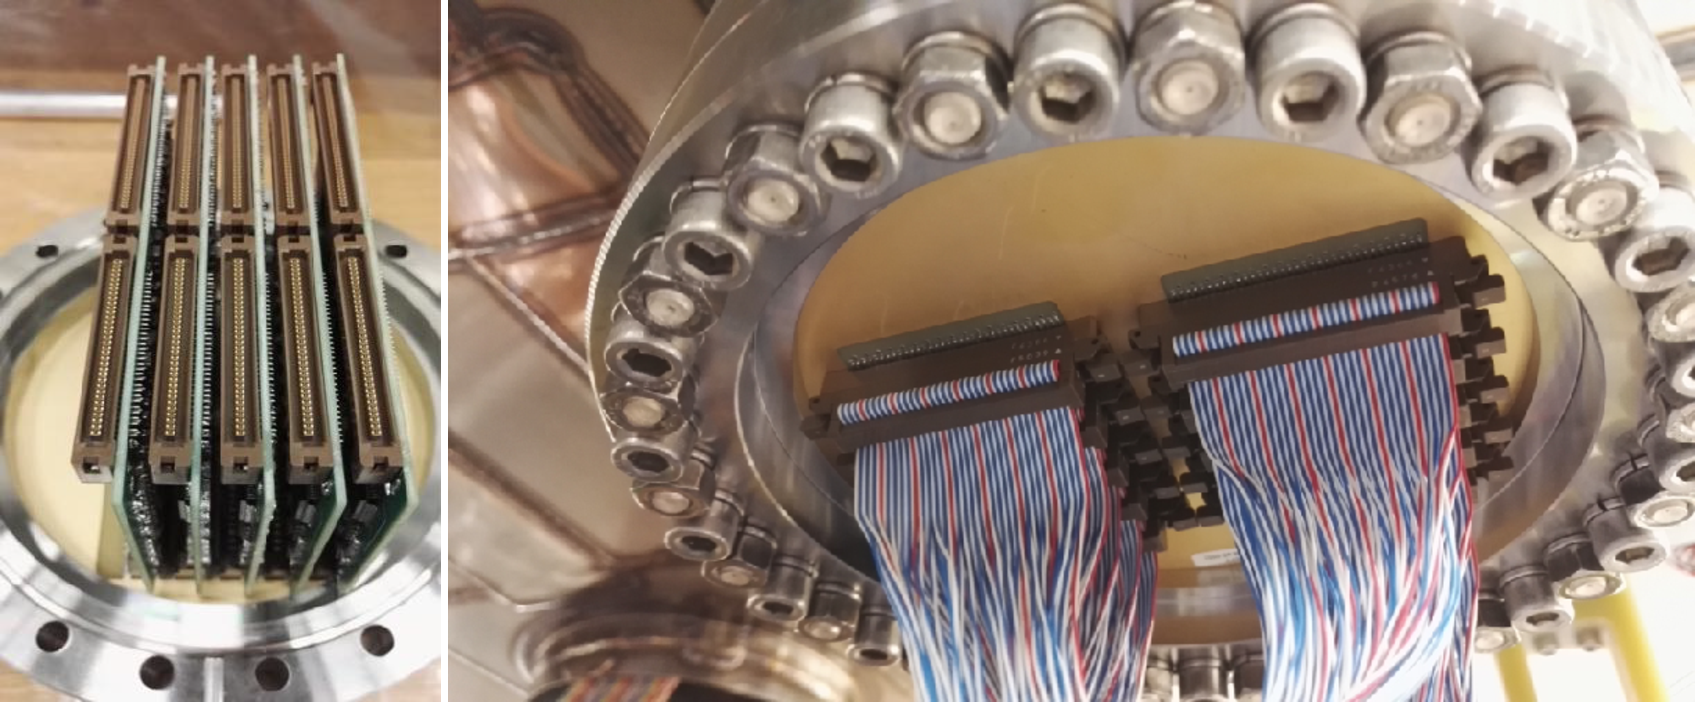
\includegraphics[width=0.8\textwidth]{dpele-sft-cold-flange}
\end{dunefigure}

%\fixme{Interfaces to light readout}
The \dword{lro} electronics is designed for negative polarity \dword{pmt} signals, with the amplitude of single photoelectrons on the input of the card between \num{1} and \SI{10}{\milli\volt}. Typically assuming a \dword{pmt} gain of \num{1E6} (no accounting for attenuation of the signals), the Catiroc ASIC can measure a range of \num{1} to \num{400} photoelectrons (\SI{160}{\femto\coulomb} to \SI{70}{\pico\coulomb}), the \dword{adc} samples from \SI{1}{\milli\volt} to \SI{1}{\volt} corresponding to \num{1} to \num{1000} photoelectrons, including the time response of the scintillator the range can increase to $\sim$\num{6000}. Increasing the gain of the \dword{pmt} to \num{1E7}, lowers the upper values by a factor of 10.

The internal noise level of the \dword{catiroc} is below \SI{0.1}{\milli\volt}. The objective for the noise level of the \dword{adc} is for each channel to have the RMS noise level greater than \SI{0.5}{LSB}, aiming for \SI{1}{LSB} \SI{0.1}{\milli\volt}.
%at 65 MHz...

%%%%%%%%%%%%%%%%%%%%%%%%%%%%%%%%%%%
\subsection{\dword{daq} System}
\label{sec:fddp-tpc-elec-intfc-daq}

The hardware interface between DP-Electronics and \dword{daq} has two components. The first interface is the \SI{10}{Gbit/s} optical fibers for data transfer between the uTCA crates and the network interface of the \dword{daq} system. The second one is a \SI{1}{Gbit/s} optical fiber that connects the \dword{daq} White Rabbit Grand Master switch to the DP electronics timing system.   

In the baseline design a given DP detector module would have \num{245} \SI{10}{Gbit/s} optical links for streaming the digitized data to \dword{daq} from the charge readout (\num{240} links) and \dword{lro} (\num{5} links) electronics housed in uTCA crates on top of the cryostat structure.  In the current specifications, the fibers are multimode OM3 fibers \cite{om3fibers} with LC-LC connectors suitable for the transmission over distances of up to \SI{300}{\metre}.  They are provided by the \dword{daq} consortium. On the side of the uTCA crate, the fibers are connected to an optical transceiver in the MCH (two SFP+ (XAUI) links) \cite{natmch}.  On the \dword{daq}, they go to the Level 1 (LV1) machines of the trigger farm, or switches, depending on the network topology adopted in the \dword{daq} system design.

The \SI{1}{Gbit/s} link going from the White Rabbit Grand Master to the DP-electronics time distribution network serves to provide the synchronization to the reference clock common for the entire FD and derived from a GPSDO (GPS-Disciplined Oscillator) clock unit installed on the surface. The clock information is distributed to the WR-MCH slave module in each uTCA crate via a set of White Rabbit switches. These switches and the interconnecting \SI{1}{Gbit/s} fibers form the timing sub-system of the DP electronics system and are included in the design of the latter. The White Rabbit synchronization protocol includes the automatic and continuous calibration of the propagation delays between the master and the connected slaves. This allows maintaining the overall synchronization between different nodes at sub-ns level. The Grand Master could be possibly located 
\begin{itemize}
\item{On surface near to GPSDO. In this case, a single fiber connects it to the DP timing system underground. The incurred latency due to the necessary fiber length to deliver the timing signals underground is automatically taken into account by the system. }
\item{Underground in CUC. In such case, the calibration of the propagation delays between GPSDO and the Grand Master would be performed manually and the timing correction would need be applied to the data afterward.}
\end{itemize} 

The design of the TPC electronics assumes that the data are streamed continuously via the \SI{10}{Gbit/s} links to the \dword{daq} system, where they are buffered until a trigger decision could be made. The triggers are to be issued by processing the buffered data in some suitable sliding time window on the trigger farm machines. The depth of the window may go up to \SI{10}{s} as needed for the definition of the Supernova triggered events. The triggers determine if the data contained in the buffers are to be written on disk. 

The software interface between \dword{daq} and the electronics systems includes the tools dealing with the data transmission and buffering: data formatting in UDP packets, compression/decompression, and exchange of the control packets.

%%%%%%%%%%%%%%%%%%%%%%%%%%%%%%%%%%%
\subsection{Cryostat and Cryogenics}
\label{sec:fddp-tpc-elec-intfc-cryo}

The interface point between the cryostat and the DP electronics system is the cryostat penetrations where the \dword{sft} chimneys are to be installed. Each penetration should accommodate the chimney whose external diameter is \SI{254}{\mm}. Each chimney has a CF-273 flange welded to its outer structure (see Figure~\ref{fig:dpele-sft-chimney-crosspipe}). After the chimney is inserted, this flange is in contact with the corresponding flange on the crossing (or penetration) pipe embedded in the cryostat structure to which it is eventually fastened. In order to avoid any leaks at this interface a CF-273 copper gasket is used to ensure the vacuum tightness.  

\begin{dunefigure}[Details of \dword{sft} chimney interface to the cryostat structure]{fig:dpele-sft-chimney-crosspipe}
{Details of \dword{sft} chimney interface to the cryostat structure.}
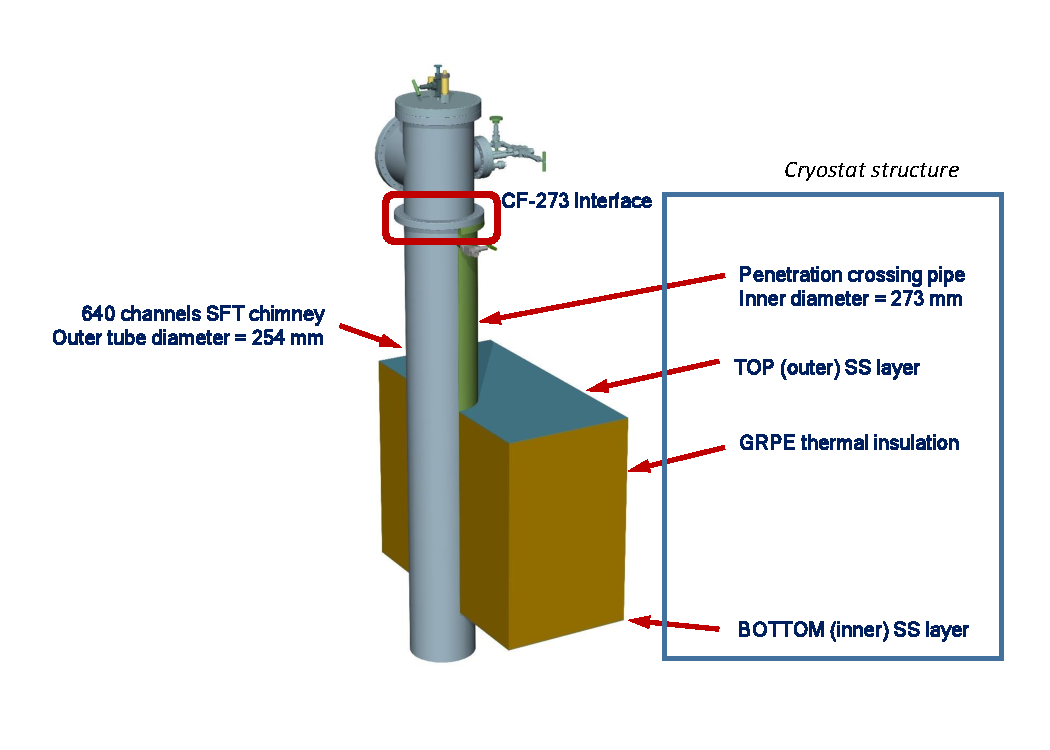
\includegraphics[width=0.7\textwidth]{dpele-sft-chimney-crosspipe}
\end{dunefigure}

Each chimney contains a heat exchanger copper coil cooled with a liquid argon. There are two (inlet/outlet) stainless steel pipe connections with \SI{10}{\mm} (\SI{12}{\mm}) inner (outer) diameter that need to be branched to the respective system for the LAr delivery and re-circulation. In addition, there is a connection for nitrogen gas line with the same pipe dimensions as those for the LAr cooling, which is used for filling the chimney after it is closed following the installation of the \dword{fe} electronics. The nitrogen line is also required for flushing the chimney in the case of an access to the \dword{fe} cards after the detector module is cooled for the operation. 

The uTCA crates for charge readout need to be installed within a short \SI{<0.5}{\meter} distance from the \dword{sft} chimneys on top of the cryostat roof. The five uTCA crates for the light readout are also placed on the roof of the cryostat at optimal locations defined by the routing of the \dword{pmt} signal cables. The required volume to accommodate the crates is roughly \SI[product-units=power]{60x50x40}{\cm}. 

%%%%%%%%%%%%%%%%%%%%%%%%%%%%%%%%%%%
\subsection{Slow Control System}
\label{sec:fddp-tpc-elec-intfc-sc}

The integration with the slow control of the low voltage power supply system for the \dword{fe} cards and uTCA crates is required to enable the remote management and monitoring (current consumption by ASICs, set voltage, etc.). In addition, the \dword{sft} chimneys contains several sensors that need to be monitored. These include a pressure transducer that measures the pressure inside the chimney and at least two temperature probes (PT1000) that monitor the gas temperature inside near the cold flange at the bottom and close to the warm flange at the top.  

%%%%%%%%%%%%%%%%%%%%%%%%%%%%%%%%%%%%%%%%%%%%%%%%%%%%%%%%%%%%%%%%%%%%
\section{Installation, Integration and Commissioning}
\label{sec:fddp-tpc-elec-install}

The installation of the TPC electronics systems proceeds in several stages. In order to cable the CRPs to the \dword{sft} chimneys, these have to be installed first prior to the start of the \dword{crp} installation inside the cryostat. After the chimneys are installed the \dword{fe} cards could be mounted on the blades and inserted. The installation of the digital electronics and uTCA crates should, however, be postponed until all of the heavy work finishes on top of the cryostat in order to ensure that the fragile components (e.g., optical fibers) are not accidentally damaged due to movement of material and large traffic of personnel. Once the uTCA crates are installed and all the digital cards are inserted, the relevant AMCs are cabled to the warm flanges of the SFTs for the charge readout and are connected to the \dword{pmt} signal cables for the light readout. Finally to complete the installation and integrate the system with the \dword{daq}, the \SI{10}{Gbit/s} and \SI{1}{Gbit/s} optical links to the \dword{daq} and WR timing network are connected. At this stage the full system is ready for commissioning. 

%%%%%%%%%%%%%%%%%%%%%%%%%%%%%%%%%%%%
\subsection{Transport and Handling}
\label{sec:fddp-tpc-elec-install-transport}
%\fixme{provide rough dimensions for boxes, chimney weights?}
%\fixme{specify that the chimneys are to be delivered for the installation underground and positioned around the cryostat on top.}

The \dword{sft} chimneys are \SI{2350}{\mm} long objects with the weight of \SI{180}{\kg}. They are shipped in wooden crates with approximate dimensions of \SI[product-units=power]{2.5x0.5x0.5}{m}. Once on site the crates are moved underground and placed on the roof of the cryostat by the UIT. The personnel from the DP electronics consortium then proceeds to unpack the crates and install the \dword{sft} chimneys. The chimneys are delivered with the cold and warm flanges already mounted and after they have been tested for leaks by one or several participating institutions.  

The boxes containing the electronic cards and uTCA crates are handled by DP electronics consortium personnel. These are foreseen to be light and could be easily carried. 

%%%%%%%%%%%%%%%%%%%%%%%%%%%%%%%%%%%
\subsection{\dword{sft} Chimneys}
\label{sec:fddp-tpc-elec-install-sft}

The installation of the \dword{sft} chimneys requires a compact gantry crane with the supports movable along the length of the cryostat. The crane itself moves along the transverse direction. The crates containing the \dword{sft} chimneys are placed along the edges of the cryostat roof. An unpacked chimney is hoisted and transported to its respective penetration crossing pipe for installation. Once in place, the chimney is fastened to the flange on the crossing pipe. The length of each chimney is about \SI{2.4}{m}. Enough overhead room should therefore be foreseen to allow to freely move the chimney with the crane along the direction transverse to the beam axis. 

In parallel with the chimney installation, the \dword{fe} cards are unpacked and mounted on the blades. This work is performed on the roof of the cryostat to avoid repackaging the blades after the assembly in order to bring them on top of the cryostat. With \dword{sft} chimneys secured in the cryostat structure, the blades with mounted \dword{fe} cards can be inserted and the chimney can be sealed. At this stage, the connections with the pipes for the liquid argon and gas nitrogen delivery could also be made, if these latter have already been installed. The pressure probes and temperature sensors can be connected to the slow control system.
 
%%%%%%%%%%%%%%%%%%%%%%%%%%%%%%%%%%%%
\subsection{Digital uTCA crates}
\label{sec:fddp-tpc-elec-install-utca}
The installation of the uTCA crates with the digital electronics should happen in the final stage of the detector installation to avoid damaging the fragile equipment. The crates are placed in their designated positions on the cryostat and connected to the power distribution network. The AMC cards and WR-MCH modules are inserted in their slots. The VHDCI cables are then attached connecting the \dword{cro} AMCs to the warm flange interface of the \dword{sft} chimneys.  The fibers from the timing system are connected to WR-MCH. 

%%%%%%%%%%%%%%%%%%%%%%%%%%%%%%%%%%%%
%\subsection{Infrastructure}
%\label{sec:fddp-tpc-elec-install-cable}

%%%%%%%%%%%%%%%%%%%%%%%%%%%%%%%%%%%
%\subsection{Integration}
%\label{sec:fddp-tpc-elec-install-integ}

%%%%%%%%%%%%%%%%%%%%%%%%%%%%%%%%%%%
\subsection{Integration within \dword{daq}}
\label{sec:fddp-tpc-elec-install-daq}
The integration of the DP TPC electronics with the \dword{daq} system requires connecting the \SI{10}{Gbit/s} fiber links to each of \num{245} uTCA crates. The connection of the timing system to the synchronization Grand Master is done via a single \SI{1}{Gbit/s} fiber link. 

The necessary software for the \dword{daq} to read and decode the data packets sent by each uTCA crate would also be provided.   

%%%%%%%%%%%%%%%%%%%%%%%%%%%%%%%%%%%
\subsection{Integration with Photon Detection System}
\label{sec:fddp-tpc-elec-install-pmt}
The cables carrying the \dword{pmt} signals from the splitter boxes need to be connected to the \dword{lro} analog electronics in each uTCA crate. The position of the crates should be optimized with respect to the layout of \dword{pmt} cables. In addition, the calibration system of the Photon Detection System has to be connected to specified inputs on the cards.

%The light read out cards will recieve the \dword{pmt} signals via their connection to the splitter boxes. Equally the calibration system of the Photon Detection System will have specified inputs to the cards.
%Anything specific apart from making cable connections? I'm not sure what should go here?

%%%%%%%%%%%%%%%%%%%%%%%%%%%%%%%%%%%
%\subsection{Calibration}
%\label{sec:fddp-tpc-elec-install-calib}

%%%%%%%%%%%%%%%%%%%%%%%%%%%%%%%%%%%
\subsection{Comissioning}
\label{sec:fddp-tpc-elec-comission}

The \dword{sft} chimneys are commissioned as a first step. This consists of evacuating and then filling them with nitrogen gas at slight overpressure with respect to the atmospheric pressure. To ensure that no damage happened to the flange interfaces during installation, the chimney vacuum tightness can be verified again at this stage by checking leak rate when the chimney is under vacuum and monitoring the nitrogen pressure once it is filled.

The electronics system can be commissioned after the installation of the uTCA crates with AMCs and the timing system are completed. The functionality of the full \dword{daq} system is not strictly required at this stage. The data from each crate could be read with a portable computer connected to the crate MCH \SI{10}{Gbit/s} or \SI{1}{Gbit/s} interface. By pulsing the \dword{crp} strips the non-functioning channels could be identified. The data quality would also be examined to ensure the correct functioning of the digital electronics and the temporal alignment of the data segments.   

%%%%%%%%%%%%%%%%%%%%%%%%%%%%%%%%%%%%%%%%%%%%%%%%%%%%%%%%%%%%%%%%%%%%
%\section{Quality Control}
%\label{sec:fddp-tpc-elec-qc}

%%%%%%%%%%%%%%%%%%%%%%%%%%%%%%%%%%%%
%\subsection{Protection and Assembly (Local)}
%\label{sec:fddp-tpc-elec-qc-local}


%%%%%%%%%%%%%%%%%%%%%%%%%%%%%%%%%%%
%\subsection{Post-factory Installation (Remote)}
%\label{sec:fddp-tpc-elec-qc-remote}


%%%%%%%%%%%%%%%%%%%%%%%%%%%%%%%%%%%%%%%%%%%%%%%%%%%%%%%%%%%%%%%%%%%%
\section{Risks and Vulnerabilities}
\label{sec:fddp-tpc-elec-risks}

The design of the DP electronics system takes into account several risks factors:
\begin{itemize}
\item{\textbf{Obsolescence of electronic components over the period of experiment}: allocation of enough spares (preferably complete cards instead of components) should be sufficient to address this issue. }
\item{\textbf{Modification to \dword{fe} electronics due to evolution in design of photon detectors}: strict and timely follow-up of the \dword{fe} requirements from the DP photon system is required.}
\item{\textbf{Damage to electronics due HV discharges or other reasons}: the \dword{fe} cards should include suitable protection components. The TVS diodes used in the current design have been sufficient to protect the electronics in \dword{wa105} detector. In addition, the cards are accessible and could be replaced if damaged. }
\item{\textbf{Overpressure in the \dword{sft} chimneys}: the \dword{sft} chimneys are equipped with safety valves that vent the excess gas in case of the sudden pressure rise. The overpressure threshold should be set low enough such that no significant damage could happen to the flanges. }
\item{\textbf{Leak of nitrogen inside the detector via cold flange}: the chimney volume would be filled with argon gas instead of nitrogen.}
\item{\textbf{Mechanical problems with \dword{fe} card extraction due to overhead clearance}: in case of insufficient overhead space it would not be possible to extract the blades from the \dword{sft} chimneys. This is addressed by making the requirement for LBNF to ensure there is always enough clearance around the chimneys.}
\item{\textbf{Data flow increase due to inefficient compression caused by higher noise}: currently there is a factor of \num{5} margin in the available bandwidth with \SI{10}{Gbit/s} MCH.}
\item{\textbf{Damage to uTCA crates due to presence of water on the roof of the cryostat}: requirement to LBNF to ensure that the cryostat surface remains dry.}
\item{\textbf{Problems with the ventilation system of the uTCA crates due to bad air quality}: normal conditions similar to any industrial environment at CERN/FNAL should be sufficient to ensure that crates function properly. Liberation of large quantities of dust due to activities in the mine are to be avoided.}
\end{itemize}
%\begin{dunetable}
%[Risks associated with DP electronics system]
%{lr}
%{tab:dpele-risks}{Risks associated with DP electronics system}
%Risk factor  &  Solution \\ \toprowrule
%Obsoleteness of electronic components over the period of experiment & \\ \colhline
%Modification to \dword{fe} electronics due to evolution in design of photon detectors & \\ \colhline
%Damage to electronics due HV discharges or other reasons & \\ \colhline
%Overpressure in the \dword{sft} chimneys & \\ \colhline
%Leak of nitrogen inside the detector via cold flange & \\ \colhline
%Mechanical problems with \dword{fe} card extraction & \\ \colhline
%Data flow increase due to inefficient compression caused by higher noise & \\ \colhline
%Damage to uTCA crates due to presence of water on the roof of the cryostat & \\ \colhline
%Problems with the ventilation system of the uTCA crates due to bad air quality & \\ \colhline
%\end{dunetable} 


%%%%%%%%%%%%%%%%%%%%%%%%%%%%%%%%%%%
% add subsections and labels if needed \subsection{}
%\label{sec:fddp-tpc-elec-safety-}


%%%%%%%%%%%%%%%%%%%%%%%%%%%%%%%%%%
%\subsection{}
%\label{sec:fddp-tpc-elec-safety}


%%%%%%%%%%%%%%%%%%%%%%%%%%%%%%%%%%%%%%%%%%%%%%%%%%%%%%%%%%%%%%%%%%%%
\section{Organization and Management}
\label{sec:fddp-tpc-elec-org}

%%%%%%%%%%%%%%%%%%%%%%%%%%%%%%%%%%%
\subsection{Dual-Phase TPC Electronics Consortium Organization}
\label{sec:fddp-tpc-elec-org-consortium}

The Dual-Phase TPC electronics consortium actually consists of seven participating institutions from France (\num{3}), Japan (\num{3}), and USA (\num{1}). The consortium leader is Dario Autiero (IPNL, France) and the technical leader is Takuya Hasegawa (KEK, Japan). The composition of the consortium along with the information for each institutional representative is provided in Table~\ref{tab:dpele-consortium-people}.
\begin{dunetable}
[DP TPC electronics consortium current participants]
{p{0.35\linewidth}p{0.25\linewidth}p{0.35\linewidth}}
{tab:dpele-consortium-people}
{DP TPC electronics consortium current participants.}   
 Institution    & Investigator & Contact \\ \toprowrule
France: APC  & Thomas Patzak & thomas.patzak@cern.ch \\ \colhline
France: IPNL  & Dario Autiero & autiero@cern.ch  \\ \colhline
France: LAPP & Dominique Duchesneau & duchesneau@lapp.in2p3.fr  \\ \colhline
Japan: Iwate University & Shinya Narita & narita@iwate-u.ac.jp  \\ \colhline
Japan: KEK    & Takuya Hasegawa & takuya.hasegawa@kek \\ \colhline
Japan: NITKC & Seiji Kasai & kasai@kure-nct.ac.jp  \\ \colhline
USA: Southern Methodist University & Thomas Coan & coan@smu.edu  \\ \colhline
\end{dunetable}

%%%%%%%%%%%%%%%%%%%%%%%%%%%%%%%%%%
\subsection{Planning Assumptions}
\label{sec:fddp-tpc-elec-org-assmp}
The present design of the DP TPC electronics system mostly relies on the elements that have already been developed and tested in \dword{wa105} detector. Commissioning of the \dword{pddp} towards the end of the year should provide some addition information, but is not expected to affect the design of principal components. Some additional improvements related to the increase in the channel density supported by AMCs  could be envisioned for the purpose of further reduction in costs. 

%%%%%%%%%%%%%%%%%%%%%%%%%%%%%%%%%%%
\subsection{WBS and Responsibilities}
\label{sec:fddp-tpc-elec-org-wbs}

The description of the WBS including the assignments of the responsible institutions is documented in DUNE-doc-5594 and provided in addendum.

%%%%%%%%%%%%%%%%%%%%%%%%%%%%%%%%%%
\subsection{High-level Cost and Schedule}
\label{sec:fddp-tpc-elec-org-cs}

\begin{dunetable}[DP TPC electronics consortium schedule]
{p{0.6\linewidth}lll}
{tab:dpele-schedule}
{DP TPC electronics consortium schedule.}
 Techincal activity  &  Days & Start date & End date \\ \toprowrule
Preparation of costing for Technical Proposal & \num{20} & 02/26/18 & 03/23/18 \\ \colhline
Initial Development of Installation Schedule & \num{20} & 02/26/18 & 03/23/18 \\ \colhline
Further Development of Installation Schedule & \num{145} & 09/03/18 & 03/22/19 \\ \colhline
Installation and Commissioning of PD-DP & \num{320} & 01/01/18 & 03/22/19 \\ \colhline
Finalization of the number of channels for \dword{lro} & \num{20} & 09/03/18 & 09/28/18 \\ \colhline
Implementation of routing for digital cards of \dword{lro} & \num{40} & 10/01/18 & 11/23/18 \\ \colhline
Preparation of final costing for TDR & \num{85} & 11/26/18 & 03/22/19 \\ \colhline
Firmware development for charge readout cards & \num{145} & 09/03/18 & 03/22/19 \\ \colhline
\end{dunetable}

The detailed cost model has been developed based on the scaling of the costs for the electronics system of \dword{pddp}. It is provided in addendum. 
Table~\ref{tab:dpele-schedule} shows an extract from the international project schedule pertaining to the technical activities of the consortium.


